\documentclass[a4paper, 12pt]{report}
\usepackage[latin1]{inputenc}
\usepackage[italian]{babel}
%\usepackage[T1]{fontenc}
\usepackage{graphicx}
\usepackage{float}
\usepackage[centertags]{amsmath}
\usepackage{amsfonts}
\usepackage{amssymb}
\usepackage{amsthm}
\usepackage{newlfont}
\usepackage{fancyhdr}
\usepackage{tesi}
\usepackage{listings}
\usepackage{hyperref}
\setcounter{secnumdepth}{5}
\setcounter{tocdepth}{3}

%-------------------------------
% DEFINIZIONE DEGLI ENVIRONMENT
%-------------------------------

\newtheorem{pro}{Problema}[chapter]
\newenvironment{prob}
    {\begin{pro}\begin{normalfont}}
    {\hfill $\spadesuit$ \end{normalfont}\end{pro}}

\newtheorem{teor}{Teorema}[section]
\newenvironment{teorema}
    {\begin{teor}\textit }
    {\hfill  \end{teor}}

\newtheorem{defn}{Definizione}[section]
\newenvironment{de}
    {\begin{defn}\begin{normalfont}}
    {\hfill $\clubsuit$ \end{normalfont}\end{defn}}

\newtheorem{theorem}{Teorema}
%-----------------------------
% CONFIGURAZIONE DELLA PAGINA
%-----------------------------

\hfuzz2pt % Don't bother to report over-full boxes if over-edge is < 2pt

\fancypagestyle{plain}{
\fancyhead{}\renewcommand{\headrulewidth}{0pt} } \pagestyle{fancy}
\renewcommand{\chaptermark}[1]{\markboth{\small CAP. \thechapter \textit{ #1}} {} }
\renewcommand{\sectionmark}[1]{\markright{\small  \thesection \textit{ #1}} {} }
\voffset=-20pt    % distanza tra il limite superiore del foglio e l'intestazione
\headsep=40pt     % distanza  l'intestazione ed il testo del corpo
\hoffset=0 pt     % misura equivalente al margine sinistro
\textheight=620pt % altezza del corpo del testo
\textwidth=435pt  % larghezza del corpo del testo
\footskip=40pt    % distanza tra il testo del corpo ed il pie' di pagina
\fancyhead{}      % cancella qualsiasi impostazione per l'intestazione
\fancyfoot{}      % cancella qualsiasi impostazione per il pie' di pagina
\headwidth=435pt  % larghezza del'intestazione e del pie' di pagina
\fancyhead[R]{\rightmark} \fancyfoot[L]{\leftmark}
\fancyfoot[R]{\thepage}
\renewcommand{\headrulewidth}{0.3pt}   % spessore della linea dell'intestazione
\renewcommand{\footrulewidth}{0.3pt}   % spessore della linea del pi�di pagina

\numberwithin{equation}{section}
\renewcommand{\theequation}{\thesection.\arabic{equation}}




%--------------------------
% MODIFICARE DA QUI IN POI
%--------------------------

\begin{document}

\raggedright

\dedicate{"Non mi fido molto delle statistiche, perch\'e un uomo con la testa nel forno acceso e i piedi nel congelatore statisticamente ha una temperatura media."\\CHARLES BUKOWSKI}

\corso{INFORMATICA} \titoloTesi{I Terremoti: Analisi dei Dati e Tecniche di Previsione} \anno{2018/2019}
\relatore{Dott. Francesco Pasquale}
\autore{Alex Mollica}


\baselineskip=21pt

\intestazione

%------------------------------------------------
% INTRODUZIONE E RINGRAZIAMENTI (NON MODIFICARE)
%------------------------------------------------
\headheight=15pt
\fancypagestyle{plain}{
\fancyhead{}\renewcommand{\headrulewidth}{0pt} } \pagestyle{fancy}
\renewcommand{\chaptermark}[1]{\markboth{\small Cap. \thechapter \textit{ #1}} {} }
\renewcommand{\sectionmark}[1]{\markright{\small  \S \thesection \textit{ #1}} {} }
\voffset=-20pt                         % distanza tra il limite superiore del foglio e l'intestazione
\headsep=40pt                          % distanza  l'intestazione ed il testo del corpo
\hoffset=0pt                           % misura equivalente al margine sinistro
\textheight=620pt                      % altezza del corpo del testo
\textwidth=435pt                       % larghezza del corpo del testo
\footskip=40pt                         % distanza tra il testo del corpo ed il pie' di pagina
\fancyhead{}                           % cancella qualsiasi impostazione per l'intestazione
\fancyfoot{}                           % cancella qualsiasi impostazione per il pie' di pagina
\headwidth=435pt                       % larghezza del'intestazione e del pie' di pagina
\fancyhead[R]{\rightmark} \fancyfoot[L]{\leftmark}
\fancyfoot[R]{\thepage}
\renewcommand{\headrulewidth}{0.3pt}   % spessore della linea dell'intestazione
\renewcommand{\footrulewidth}{0.3pt}   % spessore della linea del pi�di pagina

\pagenumbering{Roman} \tableofcontents
\newpage

\pagenumbering{arabic}

\fancyhead[R]{Introduzione} \fancyfoot[L]{Introduzione}
\fancyfoot[R]{\thepage}

\chapter*{Introduzione}
\addcontentsline{toc}{chapter}{Introduzione}

\section*{Premessa}
\addcontentsline{toc}{section}{Premessa}
Nel Capitolo \ref{background}, dove viene fornito un Background all'argomento, faccio riferimento ad enti italiani, ma il discorso sar\`a analogo per gli altri paesi, cambieranno soltanto gli enti che si occupano della raccolta e del monitoraggio dei dati e, gli enti che hanno scopi di protezione civile.\\
Quello che andr\`o a fare \`e approcciare alla predizione dei terremoti in modo diverso dall'analisi dei precursori (vedi Sezione \ref{previsione}).\\
Quindi prender\`o in analisi soltanto i dati storici dei terremoti messi a disposizione dagli enti nazionali che li raccolgono. L'idea di fondo \`e che tutto il lavoro che andr\`o a svolgere dovr\`a essere estendibile ad ogni altra realt\`a che non sia solo quella nazionale, quindi tutto \`e mirato a sviluppare uno standard che mi permetta di analizzare una grande mole di dati a prescindere della provenienza di essa.


\section*{Scopo della tesi}
\addcontentsline{toc}{section}{Scopo della tesi}
Lo scopo di questa tesi \`e sviluppare due applicativi tali che preso in input un catalogo contenente record\footnote{Oggetto o struttura dati eterogenea fatta da dati compositi, contenente quindi un insieme di campi o elementi, ciascuno dei quali identificato da un nome univoco e da un tipo di dato} rappresentati dai valori: \textbf{magnitudo}, posizione (\textbf{Latitudine} e \textbf{Longitudine}) e \textbf{data} di un terremoto, possano dare in output dei risultati utili all'analisi dei terremoti, dopo aver eseguito opportune operazioni e controlli. Questi risultati saranno rappresentati su una mappa, in quanto i terremoti stessi si verificano in una area geografica ed \`e quindi pi\`u facile in questo modo analizzare i dati; infatti la rappresentazione su mappa permetter\`a un'analisi dei dati pi\`u semplificata, grazie all'utilizzo di forme geometriche e colori che possono essere sovrapposti alla mappa.\\
L'obiettivo che mi pongo nello sviluppo di questi applicativi si pu\`o facilmente riassumere in due domande:
\begin{itemize}
    \item Quanto \`e rischiosa una determinata area geografica rispetto alle altre?
    \item Quando avverr\`a il prossimo terremoto in una determinata area geografica?
\end{itemize}

\fancyhf{} %elimina header/footer vecchi


\fancyhead[R]{\rightmark} \fancyhead[L]{\leftmark}
\fancyfoot[R]{\thepage}





%---------------------
% INCLUSIONE CAPITOLI
%---------------------
\chapter{Background}\label{background}

In questo Capitolo andr\`o a fare una panoramica generale di tutte le conoscenze necessarie per poter analizzare il lavoro della Tesi, spiegando cos'\`e un terremoto e tutti i termini tecnici che circondano questo campo di studio; continuer\`o dando un'introduzione alle attuali tecniche che si usano per fare previsione e presenter\`o i due algoritmi sviluppati a cavallo degli anni '80 e 90', gli algoritmi \textit{M8} e \textit{CN}. Successivamente spiegher\`o l'idea che voglio utilizzare per approcciare alla manipolazione dei dati, ovvero la Big Data Analytics, presentando qualche esempio passato alla storia che ha valorizzato questa disciplina, nata e cresciuta di pari passo con lo sviluppo di internet. La raccolta dei dati ha uno scopo essenziale, perch\'e molti dati non presentano immediatamente un'utilit\`a, ma questa potr\`a apparire con il passare del tempo, quindi raccogliere dati relativi un argomento specifico potrebbe aiutare a risolvere un problema completamente diverso in futuro. Infine andr\`o a spiegare la Formula che ho utilizzato per fare previsione nel mio lavoro, Formula ricavata dal Teorema della disuguaglianza di Chebyshev.

\section{Terremoto}\label{terremoto}
Un terremoto, detto anche \textbf{sisma} o \textbf{scossa tellurica}, \`e una vibrazione provocata quando masse di roccia che applicano una forza l'una contro l'altra, improvvisamente si fratturano.\\
La branca della geofisica che studia questi fenomeni \`e la \textbf{sismologia}.

\subsection{Onde Sismiche}

Le onde sismiche sono potenti oscillazioni, provocate dalla frattura delle rocce (vedi Sezione \ref{terremoto}). Queste vengono registrate dagli strumenti, e sono soggette ad analisi successive.\\
Le onde sismiche si dividono in due tipi, le \textbf{onde P}, sono le prime ad essere registrate dai \textbf{sismografi}\footnote{Strumenti per la misura e registrazione del moto del suolo, dotati di un sensore in grado di rilevare il passaggio delle onde sismiche generate da sorgenti di origine naturale o dall'attivit\`a dell'uomo.}, o dai \textbf{sismometri}\footnote{Strumenti che si differenziano dai sismografi, solo perch\'e effettuano la misura e non la registrazione del moto del suolo}, in quanto viaggiano quasi al doppio della velocit\`a dell'altro tipo, ovvero le \textbf{onde S}.\\
La differenza tra le due, oltre la velocit\`a di propagazione, \`e il modo in cui fanno vibrare il suolo. Il primo tipo, le onde P, lo fa nella direzione di propagazione, mentre il secondo tipo, le onde S, lo fa perpendicolarmente alla direzione di propagazione.\\
Il punto preciso dove le onde sismiche hanno avuto origine \`e chiamato \textbf{ipocentro}, ed \`e identificato da latitudine, longitudine e profondit\`a, mentre la sua proiezione verticale sulla superficie terrestre \`e chiamata \textbf{epicentro}, ed \`e il punto dove si verificano danni maggiori.\\

\subsection{Magnitudo}

Per misurare la grandezza di un terremoto abbiamo bisogno di un'unit\`a di misura, la \textbf{magnitudo}. Questa ci permette di renderci conto di quanta energia viene sprigionata dal terremoto. L'aumentare della magnitudo rappresenta un aumento non lineare dell'energia, o meglio, ogni qual volta la magnitudo aumenta di una unit\`a, l'energia sprigionata dal terremoto \`e circa 30 volte superiore.\\
La magnitudo viene misurata in vari modi, uno di questi \`e l'utilizzo di \textbf{sismogrammi}\footnote{Diagrammi tracciati dalle registrazioni fatte dai sismografi, che possono rappresentare lo spostamento, la velocit\`a o l'accelerazione del suolo in funzione del tempo}. Questo comporta che per avere una misura esatta, si devono confrontare vari dati. Vista l'urgenza da parte di Protezione Civile e Vigili del Fuoco, che devono intervenire in caso di terremoto, per verificare se ci sono ed eventualmente aiutare persone in difficolt\`a, viene inizialmente trasmessa una stima di magnitudo dall'\textbf{INGV}\footnote{Ente di ricerca italiano, che studia e monitora i fenomeni sismici e vulcanici} (Istituto Nazionale di Geofisica e Vulcanologia), verso gli enti sopra citati, che hanno scopi di protezione civile. Essendo questa solo una stima di magnitudo, pu\`o differire di molto dalla magnitudo definitiva.

\subsection{Pericolosit\`a e Previsione}\label{previsione}

La maggior parte dei terremoti che avvengono sulla superficie terrestre sono concentrati in zone ben precise, ossia in prossimit\`a dei confini tra due placche tettoniche, dove il contatto \`e costituito da \textbf{faglie}\footnote{Zone strette in cui le masse rocciose si muovono l'una rispetto all'altra, o anche frattura che genera il terremoto.}. In questo caso le faglie sono gi\`a preesistenti, ma questo non preclude la possibilit\`a che se ne generi improvvisamente una nuova.\\
Da ci\`o possiamo quindi renderci gi\`a conto, senza fare nessuna analisi, che le zone sopra le faglie hanno un rischio maggiore che avvenga un terremoto, rispetto alle zone dove non ci sono faglie. \cite{earthquake}\\
Le faglie pi\`u famose al mondo sono:
\begin{itemize}
    \item Faglia Alpina
    \item Faglia Atacama
    \item Faglia Chaman
    \item Faglia di Sant'Andrea
    \item Faglia di Sumatra
    \item Faglia di Messina - Giardini Naxos
    \item Faglia Gloria
    \item Faglia Nord - Anatolica
    \item Faglia Oaxaca
    \item Faglia trasforme del Mar Morto
    \item Faglia trasforme di Cefalonia
    \item Faglie SWIM
\end{itemize}
\begin{figure}[H]
   \centering
   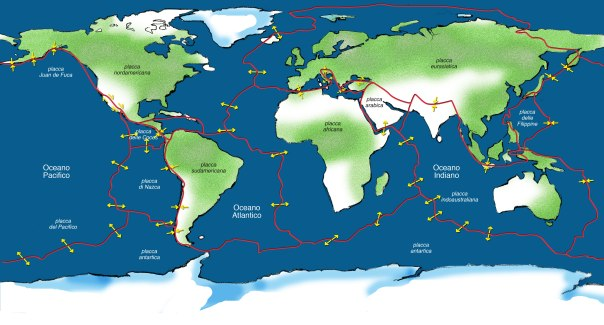
\includegraphics[width=0.835\textwidth]{images/placcheTettoniche.jpg}
   \caption{Placche tettoniche}
\end{figure}
Detto ci\`o possiamo analizzare pi\`u nel dettaglio la pericolosit\`a di una determinata zona rispetto ad un'altra. Questo discorso \`e strettamente correlato con la previsione dei terremoti.\\
La pericolosit\`a \`e quindi un'analisi della probabilit\`a che un certo scuotimento avvenga nel prossimo futuro. L'analisi pu\`o essere basata su molti fattori, ad esempio una \`e l'analisi dei \textbf{precursori}\footnote{Fenomeno anomalo che potrebbe dare un avvertimento di un terremoto imminente}, quali:
\begin{itemize}
    \item Comportamento animale;
    \item Dilatanza-diffusione;
    \item Cambiamenti in V\ped p/V\ped s;
    \item Emissioni di radon;
    \item Anomalie elettromagnetiche.
\end{itemize}
Ad oggi la validit\`a della maggioranza dei fenomeni proposti come precursori rimane indimostrata, soprattutto a causa della mancanza di osservazioni sufficientemente prolungate e sistematiche. I terremoti forti, infatti, sono eventi rari e ciascun fenomeno considerato precursore \`e caratterizzato da fluttuazioni proprie, non legate alla sismicit\`a.\\
Un altra analisi che pu\`o essere fatta per calcolare la pericolosit\`a di determinate zone, \`e l'analisi dei dati storici, che abbiamo a nostra disposizione.\\
L'analisi dei terremoti con l'obiettivo di fare previsioni, \`e oggetto di studio di migliaia di esperti, sparsi nel mondo.\\
Nel 2004 \`e stata rilasciata dall'\textbf{INGVterremoti}\footnote{Sezione dell'INGV che si occupa solo ed esclusivamente dei terremoti} la seguente mappa, che fornisce un quadro delle aree pi\`u pericolose in Italia.
\begin{figure}[H]
   \centering
   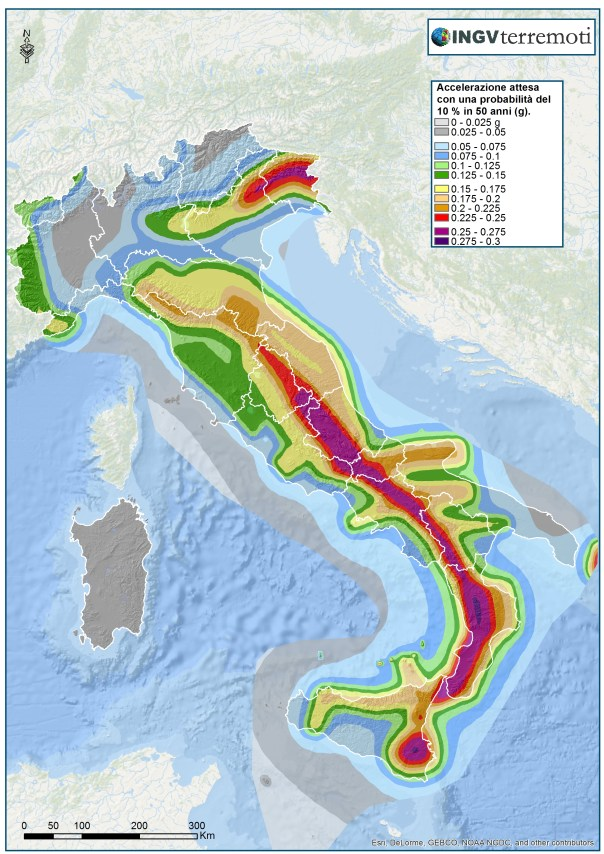
\includegraphics[width=0.5\textwidth]{images/mappaPericolosita.jpg}
   \caption{Mappa di pericolosit\`a sismica del territorio nazionale}
   \label{img:mappaPericolo}
\end{figure}
Infine l'Agenzia Spaziale Italiana ha finanziato un progetto chiamato SISMA, che utilizza tecniche di osservazione satellitari ed, in pi\`u, tiene aggiornate le previsioni a medio termine grazie a due algoritmi (CN e M8S). \cite{GiulianoFPanza}

\subsubsection{Algoritmi di previsione \textit{``M8'' e ``CN''}}

A cavallo tra gli anni '80 e '90 sono stati sviluppati due algoritmi, \textit{M8} (Keilis-Borok \& Kossobokov, 1984) e \textit{CN} (Keilis-Borok \& Rotwain, 1990) che hanno preso piede nel campo delle previsioni sismiche, sono tutt'ora utilizzati in tutto il mondo e dal Luglio 2003 anche in Italia.\\
Questi due algoritmi sono simili tra loro: utilizzano l'informazione contenuta nei cataloghi sismici, ed individuano le variazioni sismiche, che possono essere interpretate come precursori di un terremoto con magnitudo superiore ad una determinata soglia. L'analisi permette di determinare gli intervalli temporali, chiamati TIP\footnote{Times of Increased Probability (Tempi di Maggiore Probabilit\`a)}, in cui la probabilit\`a che si verifichi un terremoto con magnitudo superiore ad M0\footnote{Momento sismico. \`E utilizzato dai sismologi per misurare la quantit\`a di energia rilasciata da un terremoto}, risulta aumentata rispetto alle normali condizioni.\\
\begin{itemize}
    \item[\textbf{M8} -] Il prototipo dell'algoritmo M8 \`e stato presentato al 27\ap{o} Congresso geologico di Mosca.
L'algoritmo post-predisse il verificarsi dei terremoti di magnitudo 8.0 ed oltre in tutto il mondo, da questo deriva il nome M8.\\
Nel 1985 questo algoritmo \`e stato semplificato e riassemblato per essere applicato anche nella previsione terremoti di minore entit\`a, preservando lo schema e la definizione generale. Questa modifica \`e stata testata retroattivamente su 12 grandi terremoti verificatisi nelle regioni sismiche, principalmente nel territorio dell'URSS.\\
Durante gli anni successivi l'algoritmo M8 \`e stato testato in applicazioni per predire grandi terremoti avvenuti nel passato in altri territori. Entro il 1990, erano stati previsti in anticipo due terremoti: il terremoto di Spitak (Armenia) del 7 dicembre 1988, M = 6.9 e il terremoto di Loma Prieta (California) di ottobre 18, 1989, M = 7.1. Le previsioni furono pubblicate prima dei terremoti. \cite{algortimoM8}\\
Questo algoritmo analizza delle aree circolari, quindi i suoi rilevamenti faranno riferimento all'area nel cerchio definito inizialmente. L'algoritmo M8 scarta a priori le \textbf{scosse di assestamento}\footnote{Le scosse di assestamento sono fenomeni che si verificano dopo un terremoto di grande intensit\`a ovvero un raggruppamento di terremoti con intensit\`a minore rispetto a quello principale} rimuovendole dal catalogo preso in considerazione, in base a delle funzioni che definiscono tempo e distanza basandosi sulla grandezza del terremoto principale. Riporto di seguito la tabella che definisce queste funzioni.

\begin{figure}[H]
   \centering
   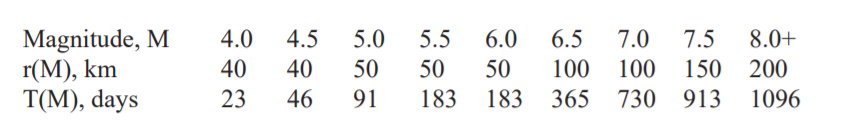
\includegraphics[width=0.850\textwidth]{images/TabellaScosseAssestamento.png}
   \caption{Tabella scosse assestamento estratta da \cite{M8Manual}}
   \label{img:tabellaScosseAssestamento}
\end{figure}

L'algoritmo decide di impostare un taglio in base alla completezza del catalogo, ovvero prendere gli eventi di una magnitudo maggiore di una certa x, questo perch\'e i dati registrati sotto quella magnitudo x sono incompleti. Una volta tolti gli eventi che si \`e deciso di scartare prende in considerazione un numero di terremoti, in base ai quali seleziona la magnitudo, ovvero mettiamo che scegliesse 20 come numero, prender\`a l'insieme di magnitudo che produce in media 20 terremoti all'anno, quindi se analizza un intervallo di 30 anni prender\`a 600 terremoti. Infine l'algoritmo calcola con delle funzioni matematiche una stima in TIP basandosi sui terremoti presi in considerazione. \cite{M8Manual}

\item[\textbf{CN} -] Un algoritmo simile all'M8 nominato precedentemente \`e il CN. Fu proposto per esaminare i precursori di sismicit\`a, dei terremoti di magnitudo $\le$ 6.4, in California e nelle regioni adiacenti come il Nevada, da cui il nome CN (California-Nevada).\\
CN \`e strutturato in modo da consentire una diagnosi dei TIP, per il verificarsi di forti terremoti.\\
L'obiettivo dell'algoritmo CN \`e quello di poter prevedere un terremoto attraverso lo studio delle attivit\`a sismiche che precedono l'avvenimento di un terremoto forte. Ci\`o \`e possibile grazie alla quantificazione degli eventi sismici, localizzati in una determinata area.\\
La quantificazione degli eventi sismici \`e ottenuta tramite un insieme di funzioni che si basano sul tempo, applicate a una sequenza di eventi avvenuti in una determinata area (escluse le scosse di assestamento). Queste funzioni quindi descrivono il livello di attivit\`a sismica, ma anche di inattivit\`a, di uno spazio-tempo, clusterizzando questi eventi.\\
Calcolate le funzioni necessarie, come ad esempio:
\begin{itemize}
    \item il livello di attivit\`a sismica;
    \item inattivit\`a sismica;
    \item variazione temporale di simicit\`a;
    \item concentrazione spaziale;
    \item clustering di terremoti.
\end{itemize}
Otteniamo il vettore P(k,t) = [p1(k,t) ... pm(k,t)] dove p(k,t) \`e una delle funzioni elencate prima.\\
Dato un tempo t e un parametro numerico r, vogliamo sapere se l'intervallo (t, t+r) appartiene a un TIP di scossa principale o di una scossa premonitrice di magnitudo M $>$ M0 nella regione k.
Questo problema \`e chiamato ``pattern recognition''. \cite{TipsCN}\\
L'allarme per il TIP \`e identificato quando il clustering \`e alto, la sismicit\`a \`e irregolare, alta e crescente (alternando intervalli di tempo di attivit\`a sismica bassa e alta). Le previsioni CN sono caratterizzate da un'incertezza temporale dell'ordine degli anni (previsioni a medio termine), poich\'e la durata dei TIP varia da pochi mesi a qualche anno e da un'incertezza spaziale di centinaia di chilometri (previsioni a medio raggio), corrispondente a un'intera singola regione monitorata. Secondo l'algoritmo, quando viene dichiarato un TIP, il forte terremoto potrebbe verificarsi in qualsiasi punto dell'area allertata, pertanto le regioni definite dovrebbero essere le pi\`u piccole possibili. \cite{algortimoCN}
\end{itemize}
Come gi\`a accennato sopra, dal Luglio del 2003 gli algoritmi CN ed M8 sono utilizzati per un collaudo sul territorio italiano. I risultati ottenuti sono i seguenti:\\
M8 ha previsto 17 dei 28 eventi di magnitudo 5.5$<$M$<$5.9 con un livello di confidenza\footnote{La definizione tecnica e completa di livello di confidenza \`e difficile da spiegare in poche righe, pertanto rimando a Wikipedia. Mi limiter\`o a fare un esempio: livello di confidenza del 99\%, presi 100 campionamenti casuali, in 99 di questi la previsione sar\`a giusta, mentre in 1 sar\`a sbagliata} superiore al 98\%.\\
CN ha previsto 12 dei 14 terremoti forti avvenuti entro le tre zone monitorate con un livello di confidenza superiore al 99\%. \cite{GiulianoFPanza}

\section{Big Data}\label{bigData}

\subsection{Cosa \`e?}
Dalla traduzione italiana abbiamo ``grandi dati'', ma io preferisco tradurlo con ``mole di dati'', questo perch\'e secondo me viene resa al meglio l'idea del concetto Big Data.\\
Big Data \`e per l'appunto una grande raccolta di dati, che nella maggior parte dei casi non si ferma nella crescita, anzi solitamente la crescita avviene in un modo molto veloce.

\subsection{A cosa serve?}\label{aCosaServono}

Per capire cosa ce ne possiamo fare di questa mole di dati prendo in considerazione un fatto accaduto nel 2009, la scoperta di un nuovo virus influenzale.\\
Questa nuova malattia fu denominata H1N1 e come molti virus si diffuse rapidamente, quindi la paura pi\`u grande era che potesse trasformarsi in pandemia. In America il CDC\footnote{Centers for Disease Control and Prevention - Centri per il Controllo e la Prevenzione delle Malattie} ordin\`o ai medici di segnalare nel pi\`u breve tempo possibile i nuovi casi di influenza. I medici fecero quanto gli fu ordinato, ma c'era un problema, che i dati erano sempre in ritardo di una o anche due settimane, questo perch\'e non tutti i pazienti segnalavano tempestivamente la malattia, in altri casi perch\`e la malattia prima di presentare i sintomi aveva un periodo di incubazione del virus che non permetteva di accorgersi di averlo contratto nell'immediato.\\
Durante l'evolversi della situazione, gli ingegneri di Google pubblicarono uno studio sulla rivista "Nature". In sostanza sostenevano di poter prevedere la diffusione dell'infulenza. Questo avveniva confrontando le ricerche digitate dagli americani nel loro motore di ricerca con i dati pubblicati dai CDC. Vennero in questo modo trovate 45 parole-chiave che presentavano una forte correlazione con i dati pubblicati dai CDC. Cos\`i a primo impatto sembra non abbiano fatto nulla di cos\`i straordinario, perch\'e producevano gli stessi risultati di previsione dei CDC, c'era per\`o una differenza sostanziale, che lo facevano in tempo reale, e non con una o due settimane di ritardo. Questo sistema messo a punto dagli ingegneri di Google si rivel\`o molto utile alle autorit\`a sanitarie per la gestione dell'epidemia.\\
Le cose che voglio prendere in considerazione di questo esempio sono le seguenti:
\begin{itemize}
    \item Gli ingegneri di Google non erano esperti in medicina, esperti in epidemie o pandemie e non erano neanche biologi o virologi;
    \item Quello che fecero gli ingegneri non fu analizzare le zone dove il virus si era sviluppato, i cosiddetti focolai;
    \item Il sistema creato prescindeva dalle ipotesi che potevano fare gli ingegneri, ad esempio vedere a cosa miravano le ricerche degli utenti.
\end{itemize}
Quindi come si evince dai punti sopra, il sistema non si basava sul ``perch\'e'' ma era comunque pi\`u efficiente nel fornire gli stessi dati pubblicati dai CDC.\\
Proprio questo \`e il concetto di Big Data, non mira a chiedersi il perch\'e avviene qualcosa, bens\`i mette insieme la mole di dati di cui si \`e a disposizione e fornisce una correlazione che in poco tempo da una risposta alla nostra domanda iniziale.\\
Noterete una certa somiglianza con la situazione in cui ci troviamo attualmente, con la nuova patologia COVID-19. Ho infatti deciso volontariamente di portare questo esempio per rispondere alla domanda posta in partenza: ``A cosa servono i Big Data?''. Attualmente Google ha messo a disposizione i Rapporti sulla Mobilit\`a della comunit\`a in formato CSV, questi saranno disponibili per un periodo di tempo limitato a condizione che i funzionari della sanit\`a pubblica ne trovino utilit\`a nel loro lavoro per fermare la diffusione del COVID-19. Chiusa questa piccola parantesi, oltre a questo esempio che ho deciso di descrivere nel dettaglio ci sono molti altri esempi interessanti dove \`e stato sfruttato il concetto di Big Data, ne cito solo un altro che ritengo importante senza entrare nel dettaglio.\\
Oren Etzioni, Professore di Informatica all'Universit\`a di Washington, che nel 2003 fece partire una start up ``Farecast'', capace di prevedere se il prezzo di un biglietto aereo sarebbe aumentato o diminuito, aveva accesso a quasi 200 miliardi di input sui prezzi dei voli.

\subsection{Big Data analytics}

L'analisi dei Big Data, come suggerisce la frase stessa, \`e un processo durante il quale si analizza la mole di dati a disposizione e si cerca una correlazione per ottenere informazioni utili al business.\\
Anche qui voglio spiegare il concetto di analisi della mole di dati portando alla luce un esempio. Amazon.com (da adesso lo chiamer\`o pi\`u semplicemente Amazon) nasce come libreria online, aveva tra i suoi dipendenti dei redattori e critici di libri, che fornivano la loro recensione e dovevano proporre nuovi titoli che Amazon aveva in vendita. Ma il fondatore e CEO di Amazon, Jeff Bezos, voleva raccomandare i libri in base ai gusti dei suoi clienti. Per questo compito decise di utilizzare i dati che aveva raccolto fino a quel momento, per\`o inizialmente approcci\`o in modo sbagliato alla sfida che si era posto, prese un piccolo campione di dati e lo analizz\`o per scoprire affinit\`a tra i suoi clienti, suggerendo cos\`i loro i libri che aveva comprato un altro cliente che risultava essere affine. Questa tecnica non ebbe un grande successo in quanto a vendite. Successivamente un programmatore che lavorava per Amazon da tempo, Greg Linden mise appunto una soluzione, questa prevedeva di correlare tra loro i prodotti, ovvero, se si era a conoscenza di quanti clienti dopo aver comprato il libro 1 compravano il libro 2, allora il libro 2 poteva essere un buon candidato a chi aveva comprato soltanto il libro 1. Anche in questo caso notiamo (vedi Sezione \ref{aCosaServono}) come non si ha a disposizione il motivo per il quale il libro 2 venisse comprato dopo il libro 1, ma si ha a disposizione comunque l'informazione, e questa informazione economicamente parlando risult\`o essere molto pi\`u importante di scovare il motivo che mette in correlazione il libro 1 con il libro 2. Infatti il computer che analizzava la mole di dati non sapeva il perch\'e un cliente che aveva comprato un libro di "Robert B. Cialdini" volesse poi comprare un libro di "Kevin Mitnick", ma sapeva soltanto che era cos\`i, quindi Amazon cominci\`o a consigliare i prodotti ai suoi clienti in modo molto coerente e trov\`o un riscontro positivo immediato nelle vendite e nel fatturato dell'azienda.\\
Questo esempio ci fa capire quindi che pi\`u \`e grande la mole di dati da analizzare e pi\`u \`e alta la probabilit\`a che il nostro algoritmo che analizza i dati far\`a previsioni attendibili, quindi possiamo affermare che \`e pi\`u importante avere a disposizione tanti dati piuttosto che meno dati pi\`u qualitativi. \cite{bigData}

\section{Disuguaglianza di Chebyshev}\label{disuguaglianzaChebyshev}
Usando la media $\mu$ e la varianza $\sigma^{2}$ della variabile casuale X si pu\`o ricavare un ``Tail Bound''\footnote{Per una variabile casuale X le ``Tails'' di X sono le parti della funzione di densit\`a discreta che sono lontane dalla sua media, quindi un ``Tail Bound'' \`e un limite a queste ``Tails''} significativamente pi\`u forte noto come Disuguaglianza di Chebyshev.

\begin{theorem}[Chebyshev theorem]
\label{ChebyshevThm}
    $\forall a > 0$\\
    $Pr(\mid X - \mu \mid \ge a) \le \dfrac{\sigma^{2}}{a^{2}}$ 
\end{theorem}

Dal Teorema \ref{ChebyshevThm} ponendo a = $\lambda\sigma$ dove:\\
$\lambda$ = numero reale positivo (che posto a 2 permette di affermare che la probabilit\`a sia sempre maggiore del 75\%)\\
$\sigma$ = deviazione standard\\
otteniamo:

\begin{equation}
    Pr(\mid X - \mu \mid \ge \lambda\sigma) \le \dfrac{1}{\lambda^{2}}
\end{equation}

Da cui svolgendo il modulo:

\begin{equation}
    Pr(\mu - \lambda\sigma \le X \le \mu + \lambda\sigma) \le \dfrac{1}{\lambda^{2}}
\end{equation}

Che equivale a scrivere:

\begin{equation}\label{chebyshev}
    Pr(\mu - \lambda\sigma \le X \le \mu + \lambda\sigma) \ge 1 - \dfrac{1}{\lambda^{2}}
\end{equation}

Quindi ho ottenuto la Formula \ref{chebyshev} che mi dice che la probabilit\`a che la variabile casuale X assuma valori compresi nell'intervallo definito tra parentesi sar\`a almeno 1 - $\dfrac{1}{\lambda^{2}}$. \cite{probAndComputing}
\include{BigData}
\chapter{Analisi dei Dati}\label{iTerremotiInItalia}
Questo Capitolo riguarda il lavoro da me svolto, dopo una descrizione dettagliata del cosa voglio fare e come lo voglio fare, vado a mettere in pratica quanto detto, entrando nei dettagli del mio lavoro di Tesi. In questo Capitolo spiegher\`o come ho cercato di rispondere alle domande che mi sono posto, sfruttando gli strumenti appresi durante questi anni di studio, ovvero la Programmazione, la Logica Matematica, la Matematica e il Calcolo delle Probabilit\`a. Questi mi hanno quindi permesso di creare due applicativi basati su approcci differenti, che vanno ad eseguire operazioni sui dati messi a disposizione dai cataloghi online e vanno a restituire in output due stime, una mirata alla probabilit\`a che avvenga un terremoto ed una mirata alla previsione dei terremoti.\\
La sezione che si occupa di terremoti dell'Istituto Nazionale di Geofisica e Vulcanologia, mette a disposizione online e scaricabile gratuitamente il CPTI15\footnote{Catalogo Parametrico dei Terremoti Italiani, versione 2.0.} \cite{CPTI15} contenente i dati storici registrati dagli strumenti raccolti negli anni dal 1000 al 2017. Il mio obiettivo \`e andare a manipolare questa banca dati resa disponibile, utilizzando algoritmi coerenti che mirino a prevedere e stimare il rischio sismico in determinate aree del paese preso in considerazione.

\section{Approccio generale e dettagli implementativi}\label{dettagliImpl}

La rappresentazione dei dati \`e un fattore molto importante per dare un senso agli stessi, pertanto di seguito spiego come ho deciso di rappresentare i dati che ho a disposizione per l'analisi dei terremoti.\\
La migliore visualizzazione che mi \`e venuta in mente per rappresentare dati di terremoti, ma soprattutto per approcciare al tema della previsione e del fattore di rischio, \`e attraverso l'utilizzo di una mappa. Ho quindi strutturato un programma che prende in input le Latitudini e Longitudini di due punti, che andranno a definire rispettivamente: il punto in basso a sinistra e il punto in alto a destra, che collegati opportunamente con 4 linee, andranno a tracciare un rettangolo sulla mappa stessa. Questa area delimitata dal rettangolo, conterr\`a l'insieme dei dati che andremo ad analizzare, pertanto ho impostato il programma in modo che scarti automaticamente i dati contenuti nel file .csv che non rientrano in quest'area. Quindi per maggiore chiarezza faccio un esempio pratico:\\ ho a disposizione 500.000 record nel file in input, ma soltanto 200.000 rientrano nell'area delimitata dalla forma geometrica che ho creato, quindi il programma scarta a priori i 300.000 inutili alla mia analisi, cos\`i da rendere pi\`u veloci eventuali operazioni ed algoritmi che andranno ad operare sui dati.\\
Una volta decisa l'area geografica, l'utilizzatore dovr\`a inserire un intero n, questo servir\`a a suddividere il rettangolo preso inizialmente in considerazione in una griglia (o matrice) costituita da nxn celle. Ci\`o permetter\`a quindi all'utilizzatore di entrare pi\`u nel dettaglio usando un intero n grande, mentre rimanere su una visione pi\`u generale usando un intero n piccolo. Questa \`e una visione del funzionamento di base del programma, di seguito spiego i due approcci che ho utilizzato per rispondere alle due domande che mi sono posto inizialmente.

\subsection{Rischio sismico}\label{rischioSismico}
Il primo approccio che chiamer\`o \textit{``Rischio sismico''} mira ad analizzare i dati con un criterio che permette di rispondere alla domanda:\\
Quanto \`e rischiosa una determinata cella rappresentante un'area geografica rispetto alle altre?

\begin{displayquote}
\textit{\textbf{$\rhd$ Divido la mappa in celle;}}\\
\textit{\textbf{$\rhd$ Sommo le magnitudo e divido per il totale;}}\\
\textit{\textbf{$\rhd$ Coloro la mappa in base alla pericolosit\`a della cella con somma massima.}}
\end{displayquote}

Per fare questo ho agito con un criterio logico descritto di seguito. Come spiegato nella sezione precedente (vedi Sezione \ref{dettagliImpl}) ho a disposizione un'area delimitata da una griglia nxn. Inizialmente ho preso in considerazione gli eventi sismici del CPTI15, che sono poco meno di 5000 record, per cominciare a strutturare l'algoritmo per analizzare i dati (naturalmente questo primo database che ho utilizzato non permette una Big Data analytics, questo perch\`e i record contenuti sono relativamente pochi, ma una volta definito l'approccio e testato il funzionamento, il programma potr\`a prendere in maniera dinamica i dati, non sar\`a quindi un problema analizzare cataloghi con una mole di dati tale da poter essere definita una Big Data analytics). L'obiettivo che mi sono posto \`e quello di andare a colorare ogni cella della griglia in base alla somma delle magnitudo avvenute nelle rispettive celle. Per fare questo ho utilizzato tre colori, il verde, il giallo ed il rosso; sono andato poi anche a sfruttare l'opacit\`a del colore per avere una scala pi\`u dettagliata senza utilizzare pi\`u di tre colori. Quindi una volta completato l'algoritmo l'output che otterr\`o sar\`a una mappa dell'Italia, con una griglia nxn dove ogni cella ha un colore; se la cella ha un fattore di rischio basso, sar\`a colorata di verde chiaro, se ha un fattore di rischio alto sar\`a colorata di un rosso pi\`u scuro.\\
Ora vado ad analizzare nel dettaglio il criterio che permette di stabilire il fattore di rischio, che verr\`a utilizzato per colorare le celle della mappa.\\
Presa la matrice che rappresenta la griglia avente nxn celle, scorro i dati che sono memorizzati nel file .csv in ordine cronologico non decrescente (condizione necessaria, utile pi\`u tardi nel secondo approccio), quindi per ogni record se il terremoto \`e avvenuto nella cella i-esima incremento il valore della cella del valore della magnitudo del terremoto i-esimo, pertanto alla fine avr\`o una matrice contenente in ogni cella la somma delle magnitudo dei terremoti che si sono verificati dentro quella cella. A questo punto sommo il valore di tutte le celle, ed avr\`o la somma complessiva delle magnitudo dei terremoti avvenuti in tutte le celle, ora dividendo il valore di ogni cella per questa somma ottenuta e sostituendolo al valore precedente che aveva ogni cella, avr\`o una matrice che somma a 1.\\
Per colorare la mappa in maniera dinamica, ho deciso di stabilire un fattore di rischio che va da 0.0 a 100.0, quindi prendere il valore massimo contenuto tra tutte le celle ed assegnargli un fattore di rischio di 100.0 su 100.0. Questo comporter\`a che per ogni possibile n scelto in input, ci sar\`a sempre una cella con fattore di rischio massimo e tutte le altre saranno colorate di conseguenza in output. La colorazione sar\`a rapportata al fattore di rischio nel seguente modo:
\begin{itemize}
\item Fattore di rischio $\le$ 10 colore verde opacit\`a 30\%
\item Fattore di rischio $>$ 10 e $\le$ 20 colore giallo opacit\`a 30\%
\item Fattore di rischio $>$ 20 e $\le$ 30 colore giallo opacit\`a 40\%
\item Fattore di rischio $>$ 30 e $\le$ 40 colore giallo opacit\`a 50\%
\item Fattore di rischio $>$ 40 e $\le$ 50 colore rosso opacit\`a 30\%
\item Fattore di rischio $>$ 50 e $\le$ 70 colore rosso opacit\`a 40\%
\item Fattore di rischio $>$ 70 colore rosso opacit\`a 60\%
\end{itemize}

\subsubsection{Risultati}

Di seguito vediamo una serie di test effettuati lanciando il primo programma che si basa sull'approccio \textit{``Rischio sismico''}:

\begin{figure}[H]
   \centering
   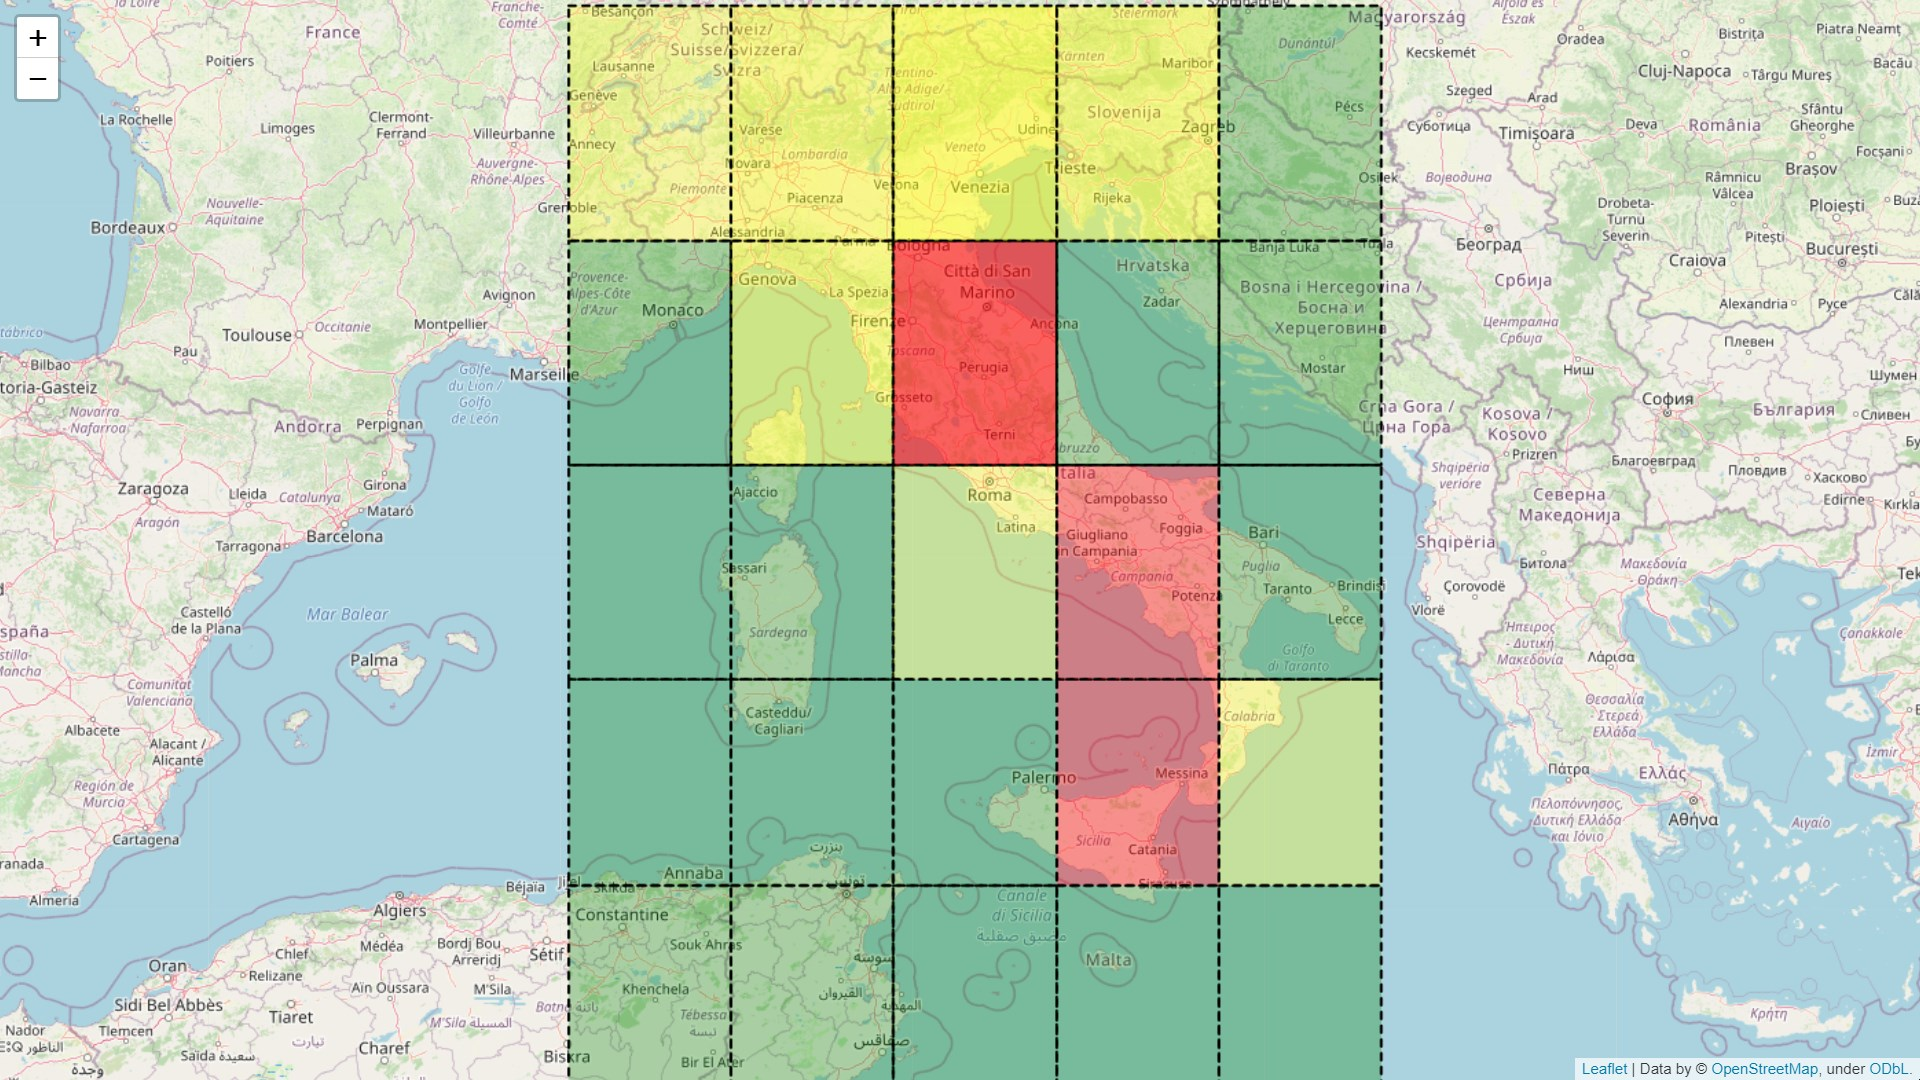
\includegraphics[width=0.835\textwidth]{images/5x5_CPTI15.jpg}
   \caption{Griglia 5x5 con DB CPTI15}
\end{figure}

Questo \`e l'output del programma se lanciato prendendo in considerazione l'Italia, con la base dati CPTI15, e con n=5. Come si evidenzia abbiamo una cella con fattore di rischio 100 che \`e quella posizionata nel centro Italia e le altre che si basano su quella come riferimento, quindi le due con fattore di rischio, subito precedenti al massimo sono le due che vediamo nella zona del meridione e tra Calabria e Sicilia.

\begin{figure}[H]
   \centering
   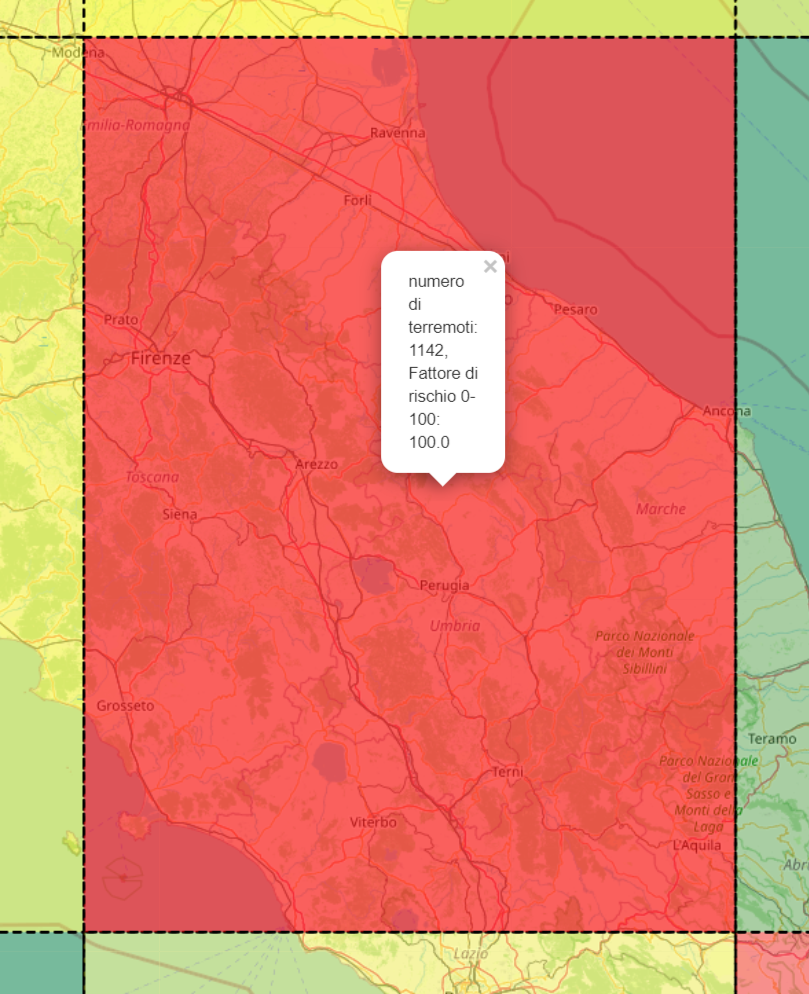
\includegraphics[width=0.600\textwidth]{images/FattoreDiRischio5x5_CPTI15_centro.png}
   \caption{Griglia 5x5 con DB CPTI15, zoom dettaglio centro Italia}
   \label{fig:zonaCentrale}
\end{figure}

\begin{figure}[H]
   \centering
   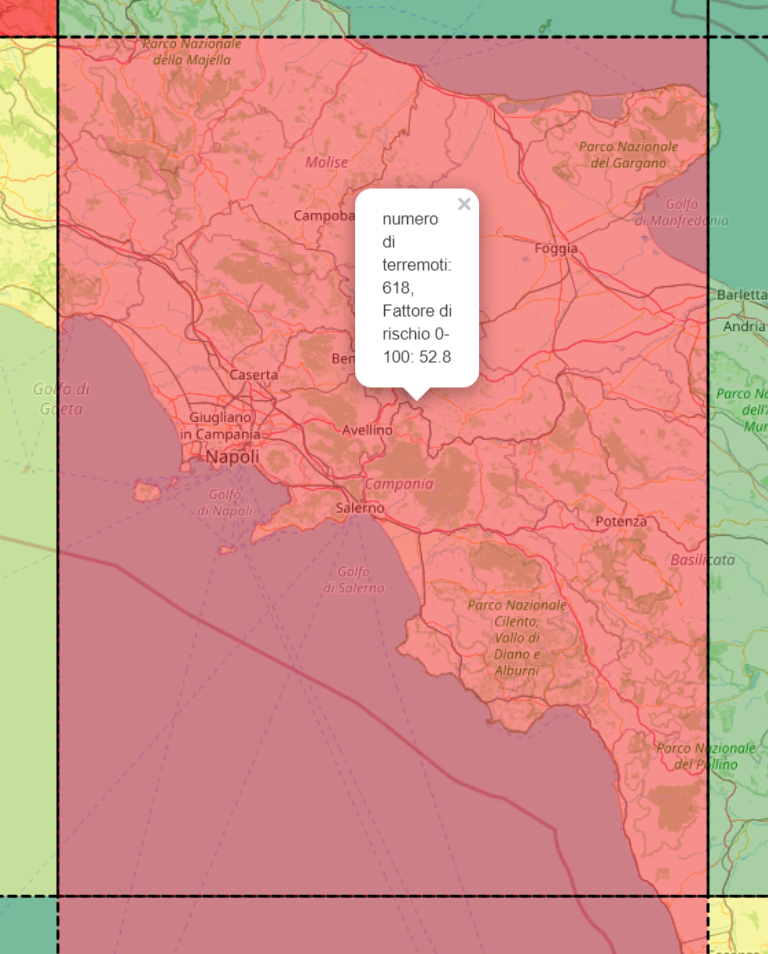
\includegraphics[width=0.600\textwidth]{images/FattoreDiRischio5x5_CPTI15_meridione.png}
   \caption{Griglia 5x5 con DB CPTI15, zoom dettaglio Italia meridionale}
   \label{fig:zonaMeridionale}
\end{figure}

Di seguito ci sono altri due esempi di come il programma permette di entrare pi\`u nel dettaglio, andando ad analizzare due casi specifici, nella Figura \ref{fig:zonaCentrale} possiamo vedere un pop-up sulla cella relativa alla zona centrale, con fattore di rischio maggiore, che ci dir\`a quanti terremoti sono avvenuti in questa cella e il relativo fattore di rischio. Nella successiva Figura \ref{fig:zonaMeridionale} possiamo vedere come il fattore di rischio sia poco pi\`u della met\`a rispetto al massimo, quindi avremo la cella colorata di rosso con un'opacit\`a del 40\%.

\begin{figure}[H]
   \centering
   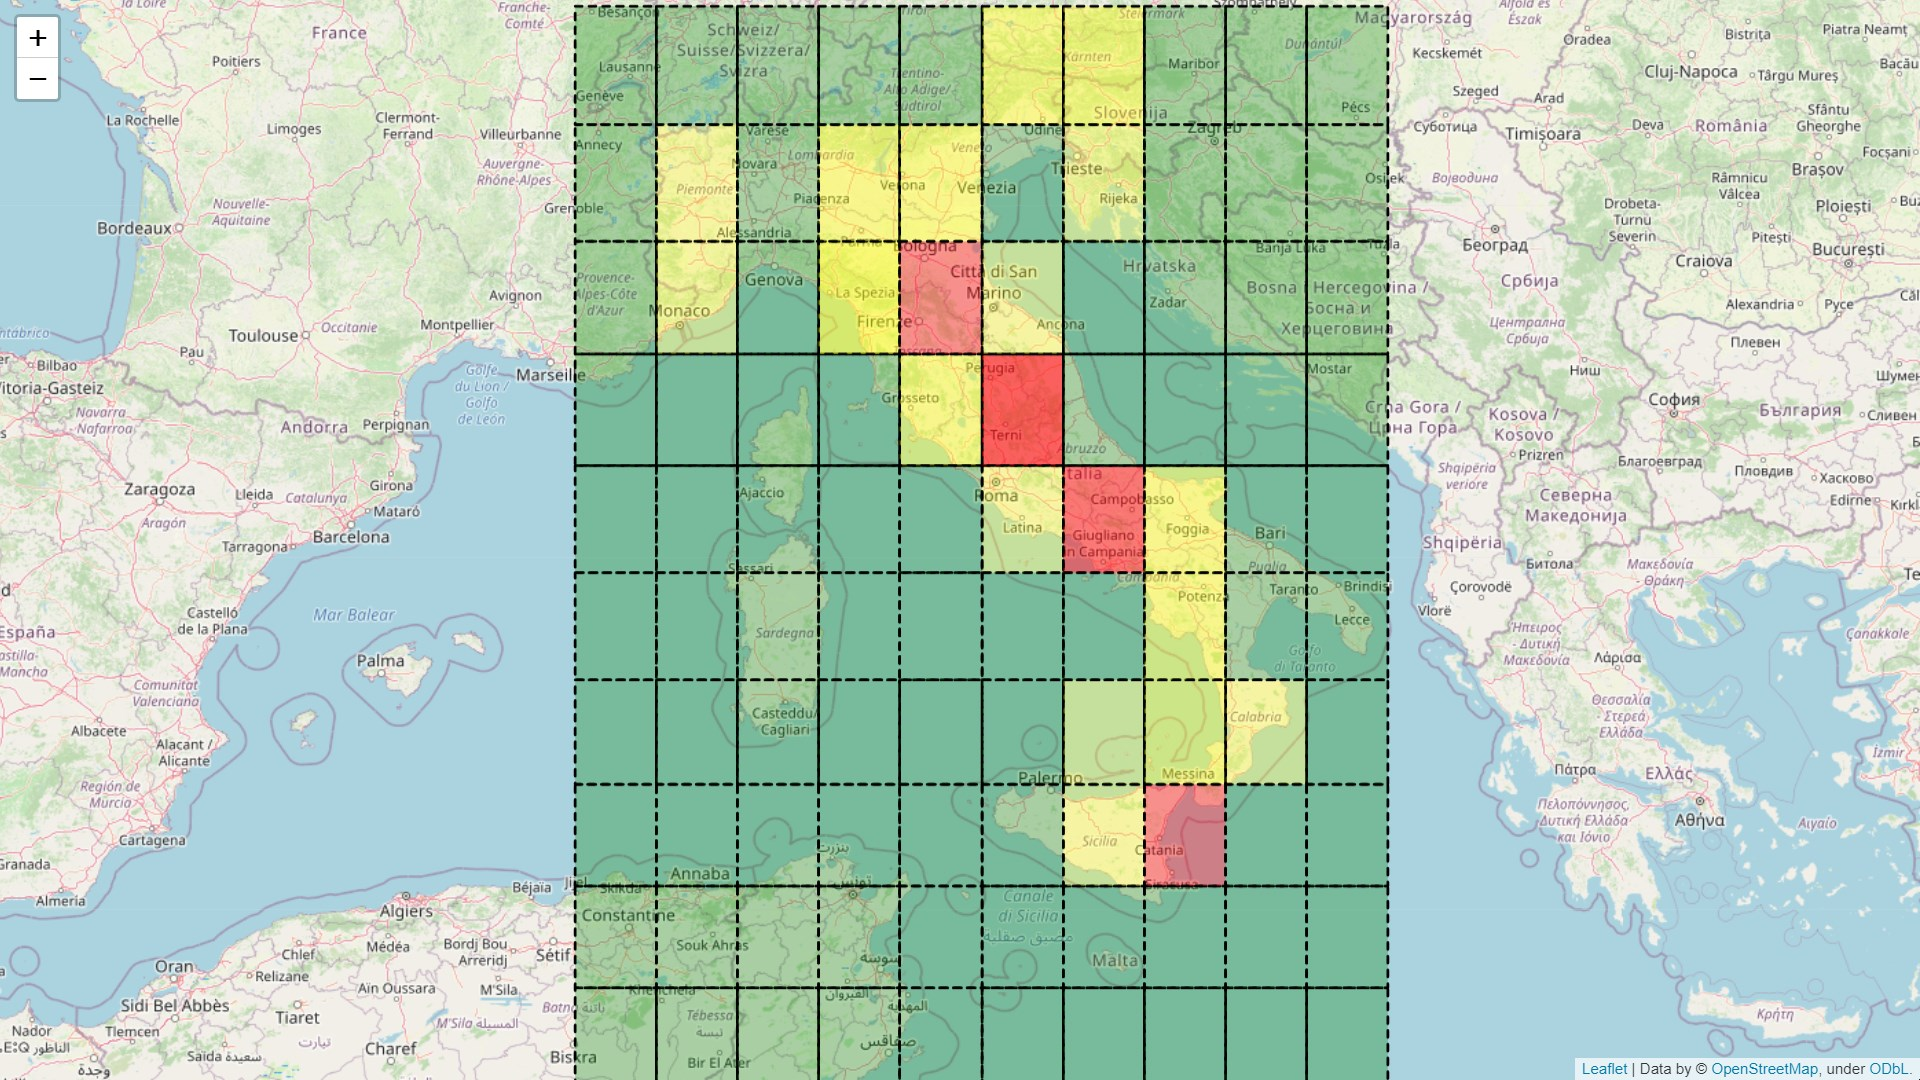
\includegraphics[width=0.835\textwidth]{images/10x10_CPTI15.jpg}
   \caption{Griglia 10x10 con DB CPTI15}
   \label{fig:10x10CPTI15}
\end{figure}

\begin{figure}[H]
   \centering
   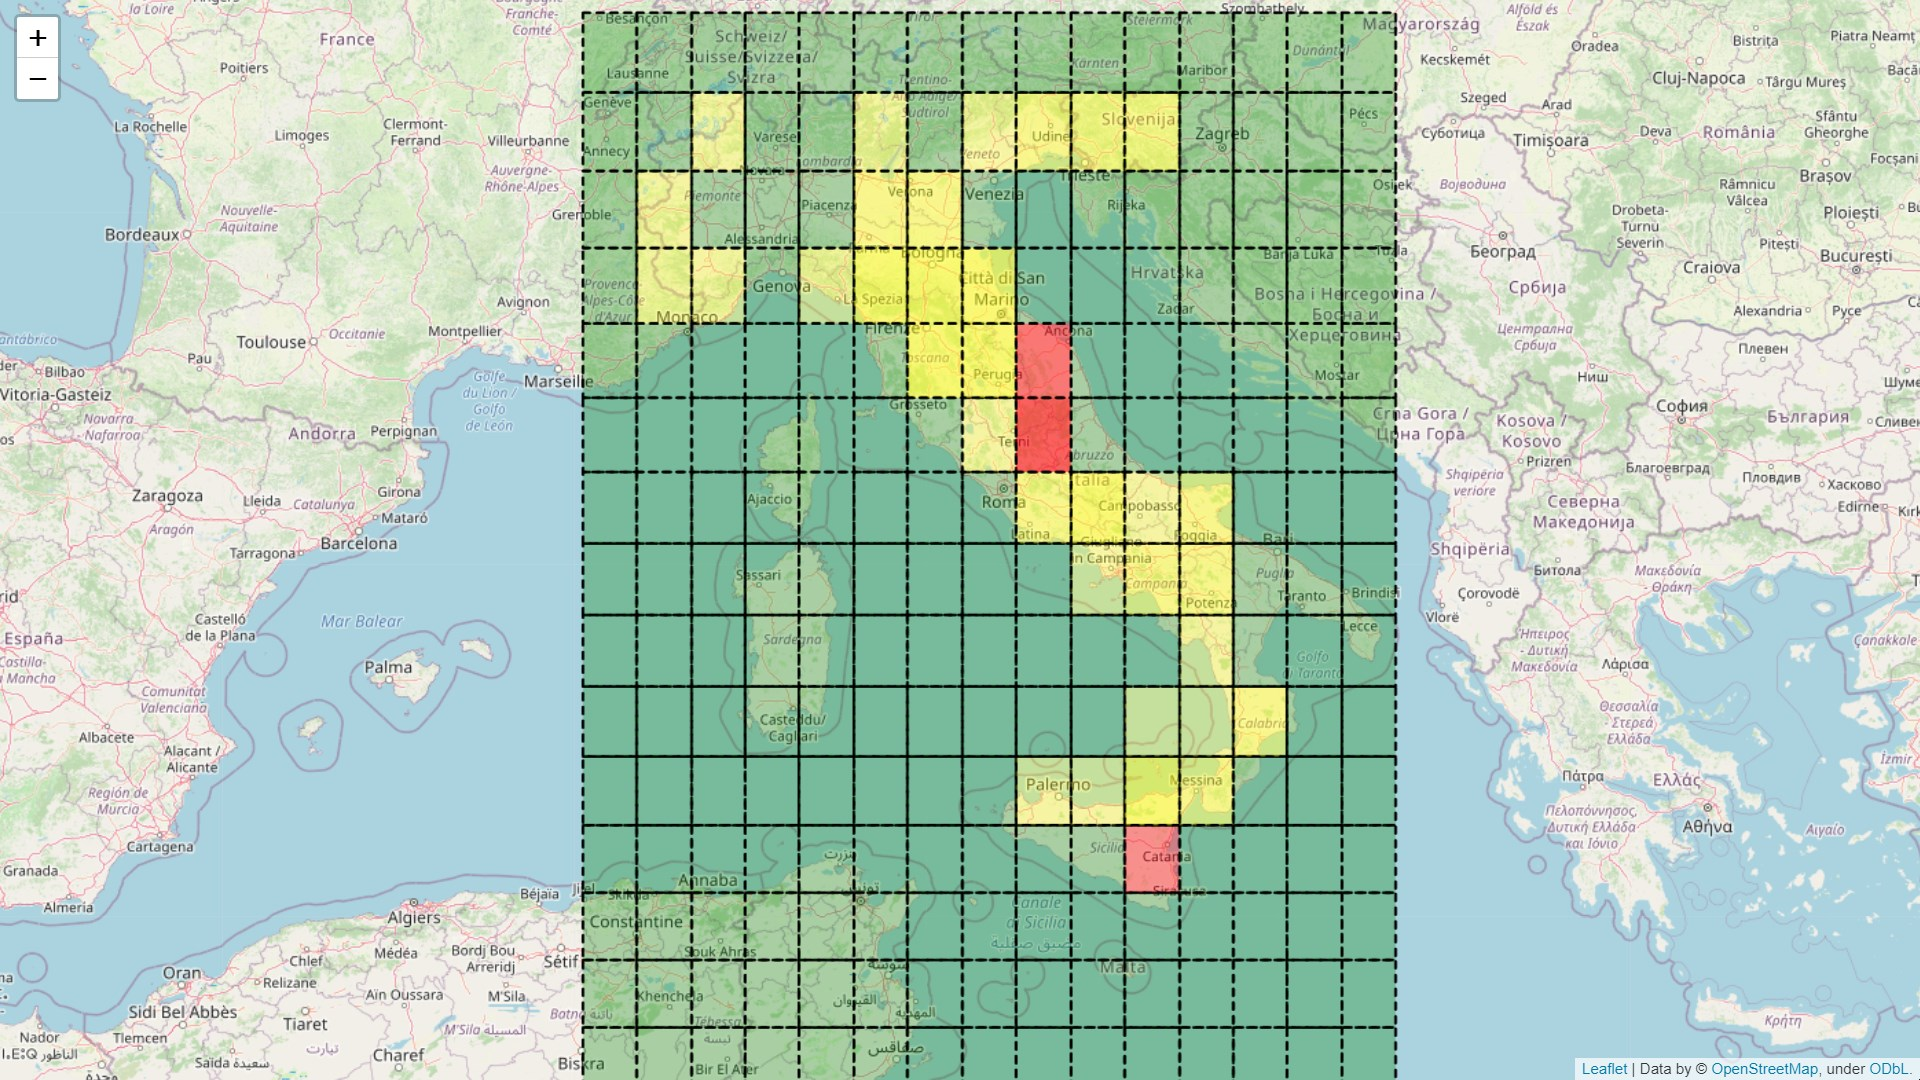
\includegraphics[width=0.835\textwidth]{images/15x15_CPTI15.jpg}
   \caption{Griglia 15x15 con DB CPTI15}
   \label{fig:15x15CPTI15}
\end{figure}

Nelle Figure \ref{fig:10x10CPTI15} e \ref{fig:15x15CPTI15} sopra vediamo come cambiando la n in input, rispettivamente in 10 e 15, otteniamo due griglie aventi rispettivamente 100 celle e 225 celle. Questo permette di fare un analisi pi\`u dettagliata restringendo cos\`i l'area ricoperta da ogni cella.

\begin{figure}[H]
   \centering
   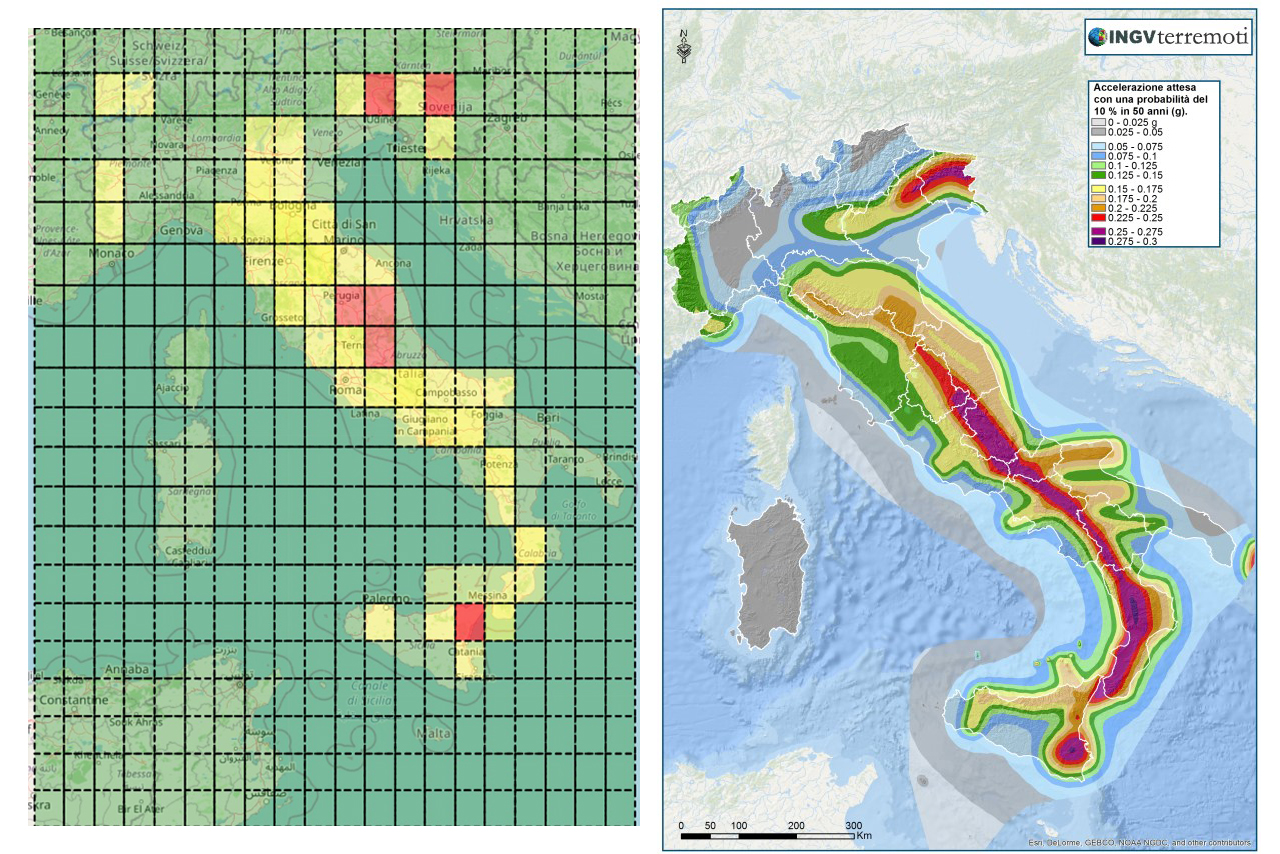
\includegraphics[width=0.835\textwidth]{images/mappaPericolositaVs20x20.jpg}
   \caption{Confronto griglia 20x20 con mappa pericolosit\`a sismica del territorio nazionale}
   \label{fig:20x20vsWarningMap}
\end{figure}

Ora ho voluto prendere in considerazione l'output del programma con n=20 come input, avendo cos\`i ristretto ancor di pi\`u l'area di ogni cella. Ho quindi messo a confronto la griglia di 400 celle con la mappa di pericolosit\`a sismica del territorio nazionale vista in precedenza (vedi Figura \ref{img:mappaPericolo}), questo porta alla luce come gi\`a l'approccio pi\`u logico, ovvero la somma delle magnitudo degli eventi sismici avvenuti in ogni cella dia un risultato molto vicino alla mappa di pericolosit\`a sismica attualmente pubblicata dall'INGV. Come detto in precedenza questo programma non tiene in considerazione precursori sismici, bens\'i si basa solo ed esclusivamente sull'analisi dei dati storici a disposizione. L'analisi appena fatta non permette di poter affermare nulla, se non che nelle celle rosse in passato sono avvenuti pi\`u eventi sismici o comunque eventi sismici di maggiore entit\`a rispetto le altre. Ora per provare il programma e testarne il comportamento con una mole di dati superiore andr\`o ad utilizzare il database messo a disposizione dell'USGS\footnote{Agenzia scientifica del Governo degli Stati Uniti, suddivisa in dipartimenti che si occupano delle seguenti aree scientifiche: biologia, geografia, geologia e idrologia} (United States Geological Survey - Agenzia per la Sorveglianza Geologica degli Stati Uniti), contenente 1.800.000 eventi sismici, dei quali circa 21.000 avvenuti nel territorio italiano, negli anni 1960-2017.

\begin{figure}[H]
   \centering
   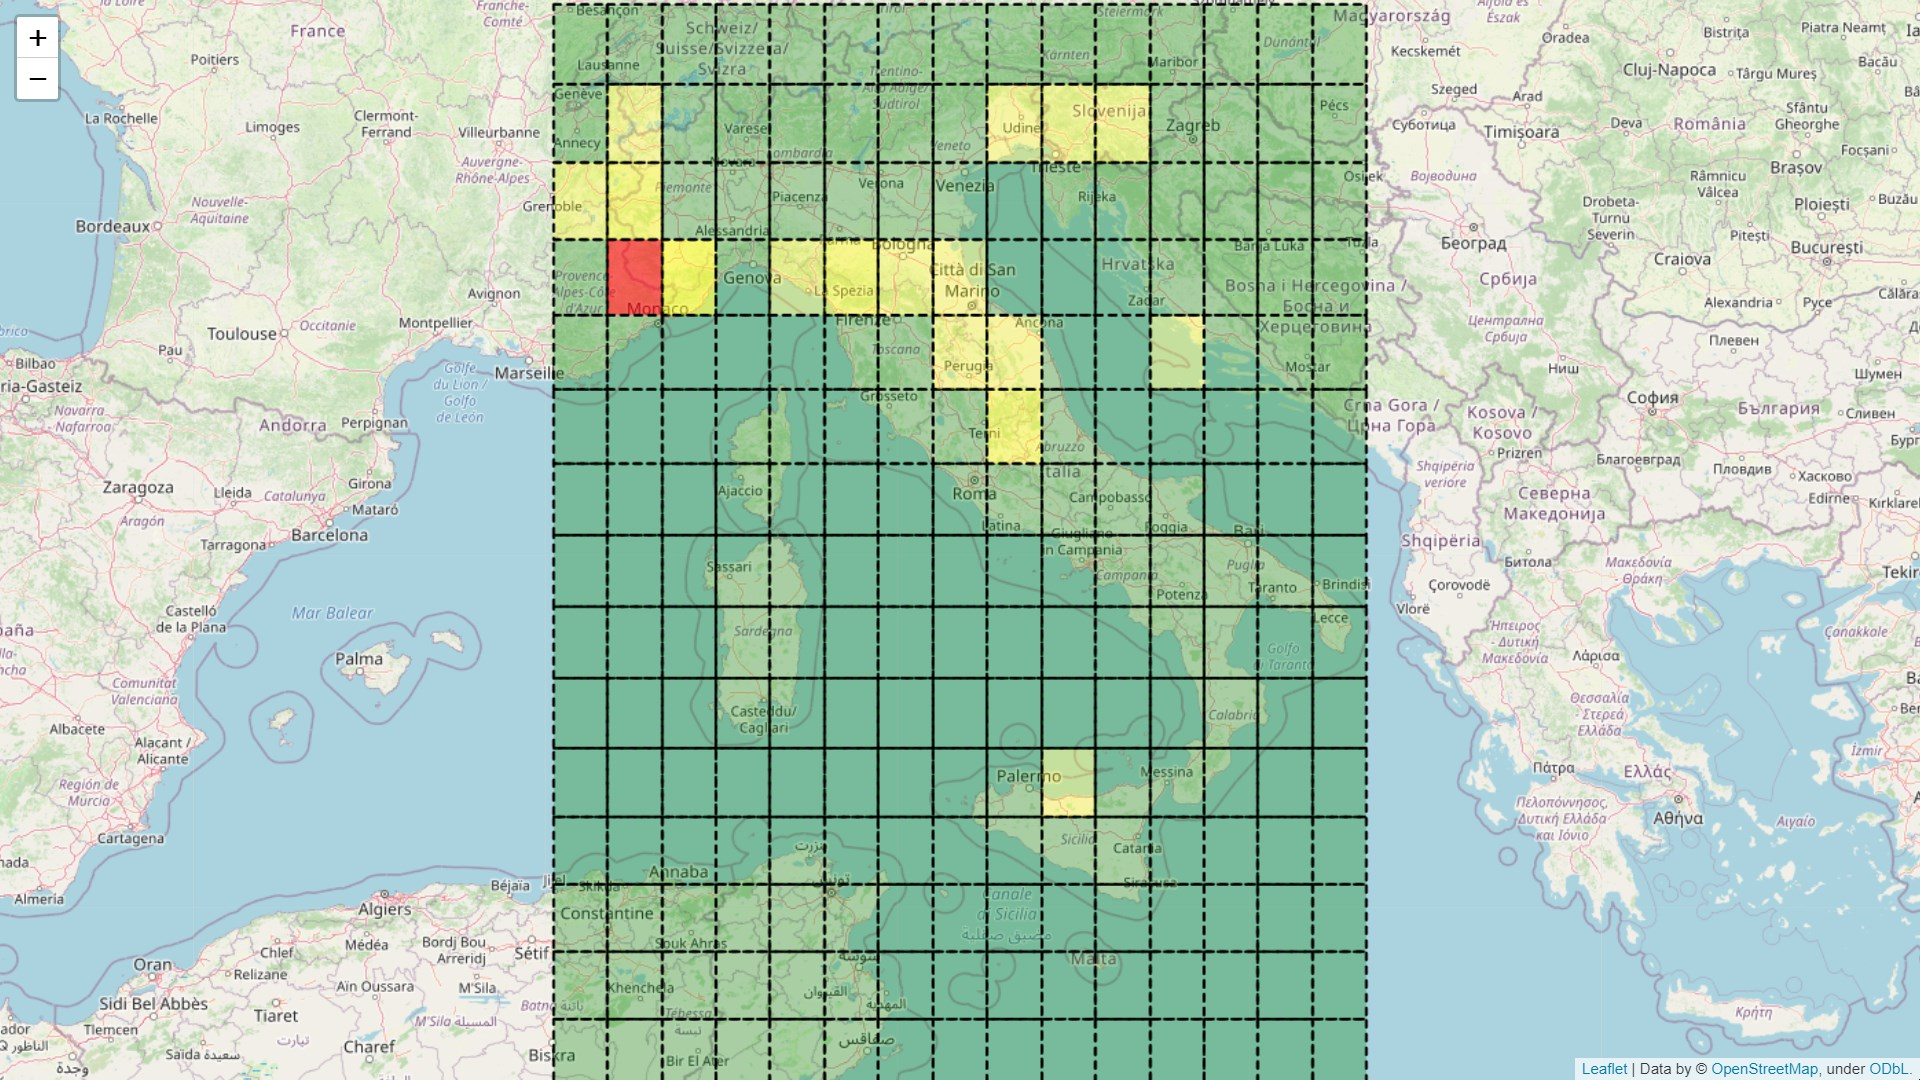
\includegraphics[width=0.835\textwidth]{images/15x15_USGS.jpg}
   \caption{Griglia 15x15 con DB USGS}
   \label{fig:15x15USGS}
\end{figure}

\begin{figure}[H]
   \centering
   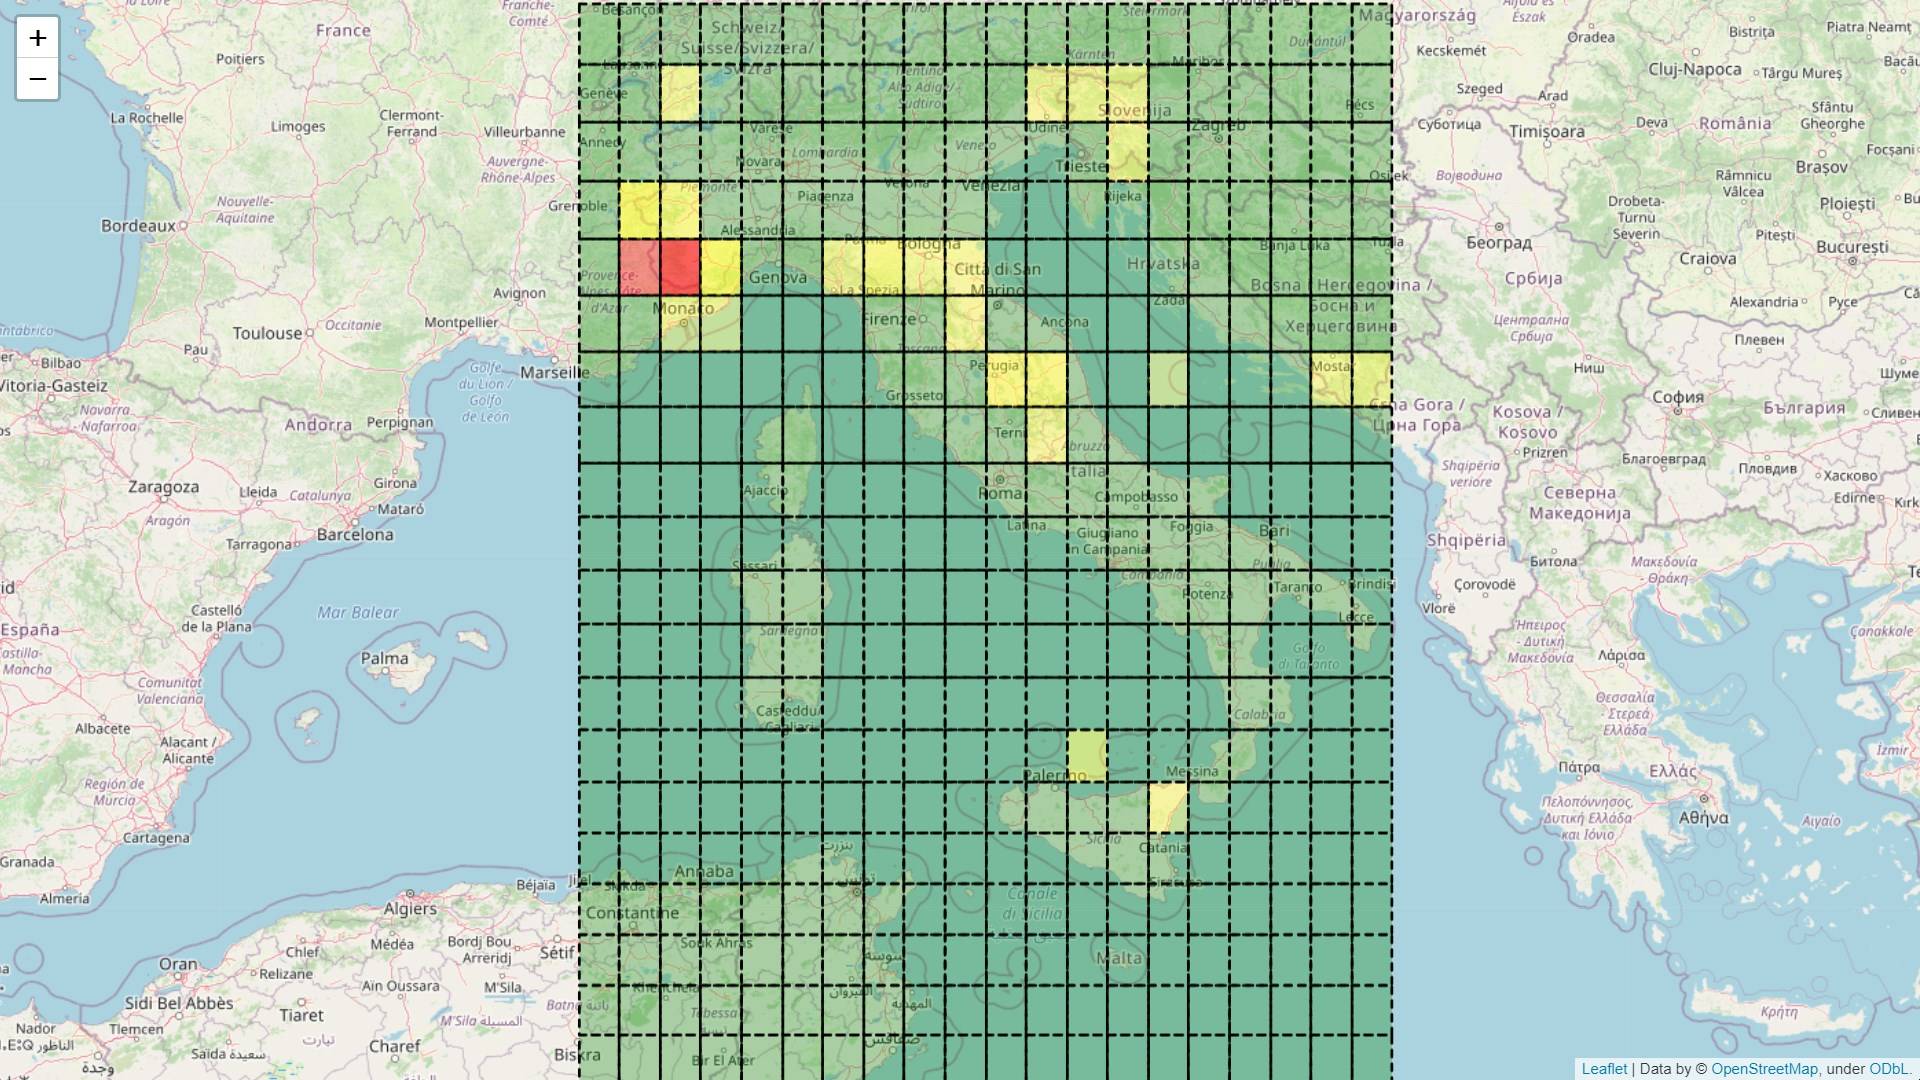
\includegraphics[width=0.835\textwidth]{images/20x20_USGS.jpg}
   \caption{Griglia 20x20 con DB USGS}
   \label{fig:20x20USGS}
\end{figure}

Notiamo subito una differenza grafica tra i dati del CPTI15 e dello USGS. Questo avviene perch\'e le celle vengono confrontate con quella avente fattore di rischio maggiore rispetto alle altre, pertanto nella Figura \ref{fig:15x15USGS} abbiamo 6240 eventi sismici avvenuti tutti nella cella 2x4 mentre nelle altre celle, a partire da quelle colorate di giallo scuro abbiamo dai 2200 eventi in gi\`u. Questo rimane uguale se andiamo ad aumentare la n in input ponendola uguale a 20, infatti la situazione nella Figura \ref{fig:20x20USGS} \`e pressocch\'e simile, se non che la cella con fattore di rischio massimo \`e la 3x5 con 4254 eventi sismici.\\
L'ultimo risultato che voglio portare alla luce \`e il confronto tra le mappe con griglia 20x20 generate dallo USGS e dal CPTI15. Come si vede, le celle precedentemente rosse sulla mappa relativa al CPTI15 sono diventate gialle, perch\'e cambiando la base dati di riferimento \`e cambiata anche la cella di riferimento con fattore di rischio maggiore.

\begin{figure}[H]
   \centering
   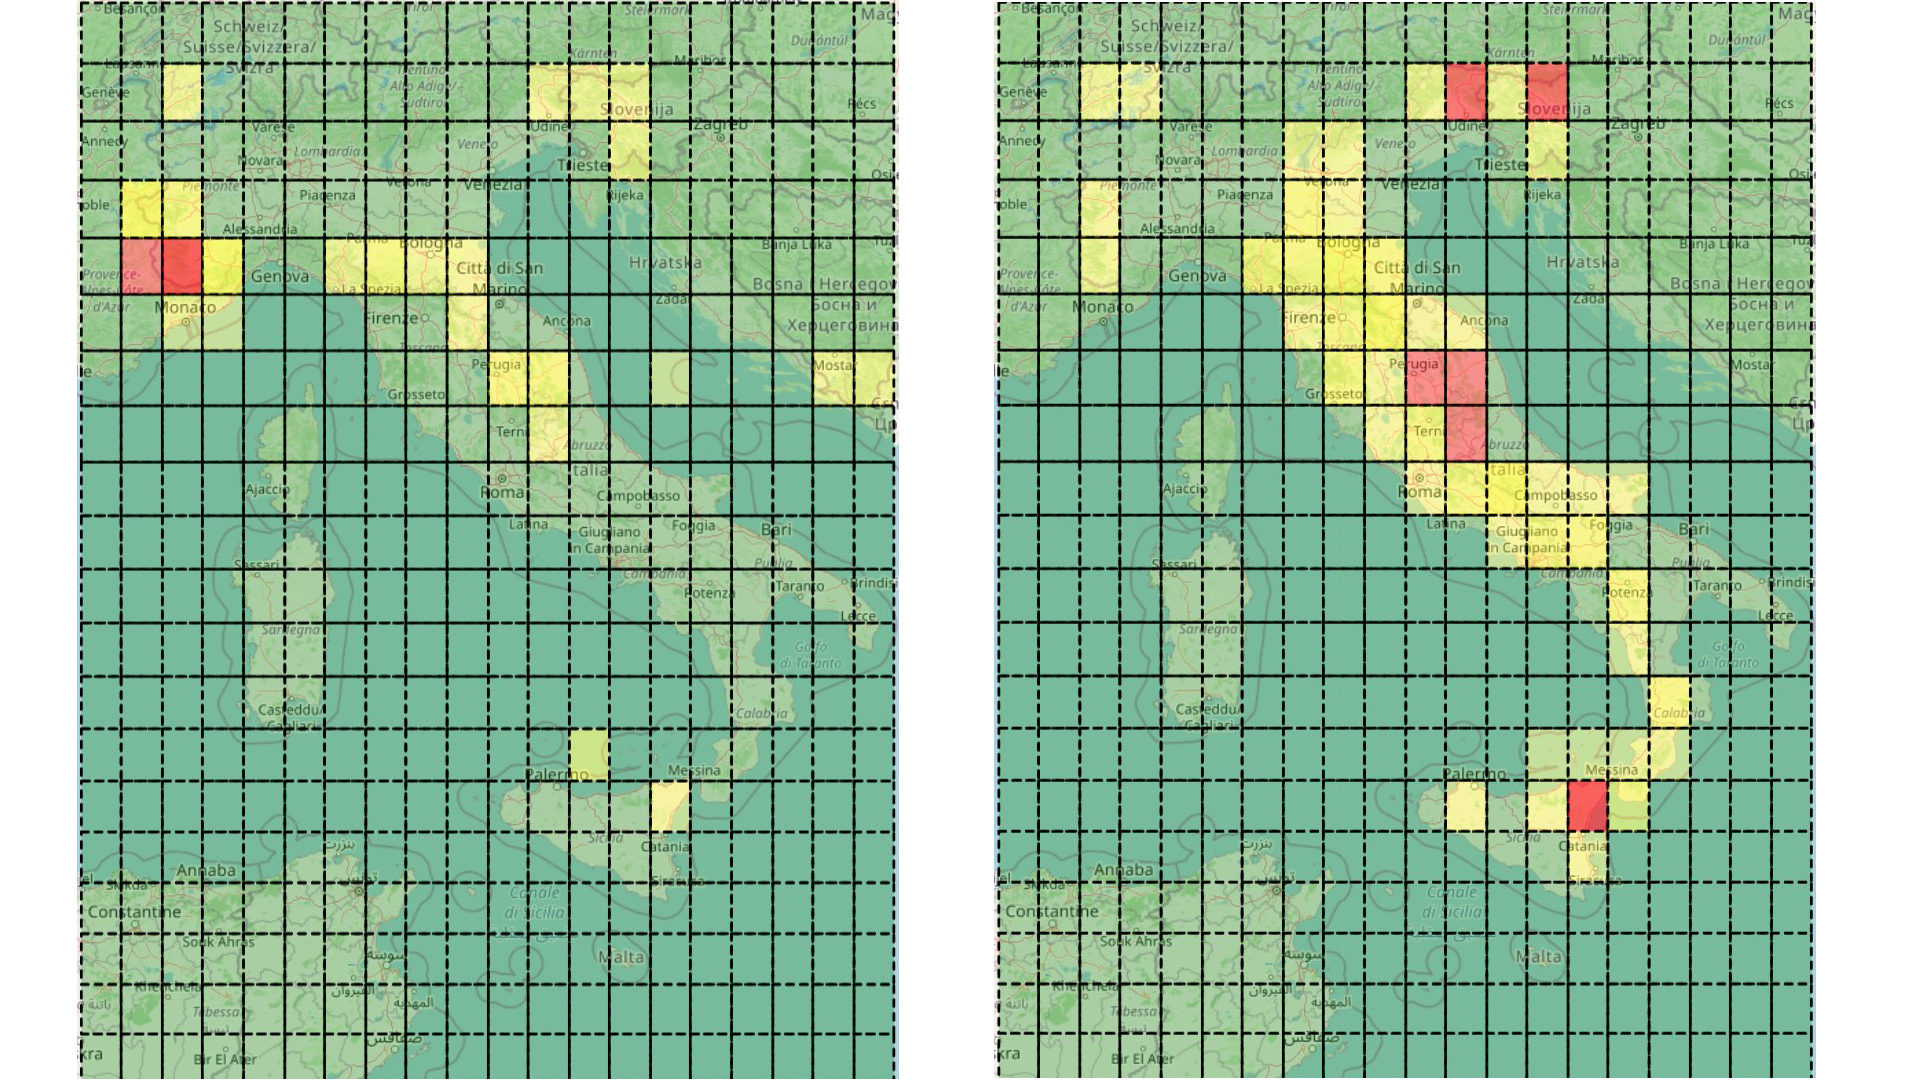
\includegraphics[width=1.0\textwidth]{images/20x20_USGS_vs_CPTI15.jpg}
   \caption{Confronto griglia 20x20 con DB USGS e griglia 20x20 con DB CPTI15}
\end{figure}

\subsection{Previsione}
Il secondo approccio che chiamer\`o \textit{Previsione} mira ad analizzare i dati con un criterio che permette di rispondere alla domanda:\\
Quando avverr\`a il prossimo terremoto con magnitudo maggiore di x, con 0$\le$x$\le$10, nella cella i-esima?\\
Per fare questo vado a tracciare uno schema di funzionamento dell'algoritmo:

\begin{displayquote}
\textit{\textbf{$\rhd$ Divido la mappa in celle;}}\\
\textit{\textbf{$\rhd$ Estraggo l'intervallo di tempo tra i terremoti con magnitudo maggiore di m, occorsi in ogni cella;}}\\
\textit{\textbf{$\rhd$ Calcolo media e varianza dei giorni tra un terremoto e il successivo;}}\\
\textit{\textbf{$\rhd$ Assumendo che l'intervallo di tempo che intercorre fra due terremoti si comporti come una variabile casuale X, stimo un intervallo di confidenza con la disuguaglianza di Chebyshev.}}
\end{displayquote}

Come \`e chiaro dai Capitoli precedenti, la previsione dei terremoti \`e un campo di studio molto ampio che vede impegnate persone di ogni paese nella ricerca di tecniche predittive. Nonostante questo attualmente la previsione si limita a dare delle stime a medio/lungo termine, questo per evidenziare che la domanda alla quale vorrei rispondere attraverso il secondo approccio nasconde insidie nelle quali \`e pericoloso avventurarsi. Quindi per fare un'affermazione che risponda alla domanda dovrei avere una certezza che non mi \`e possibile avere, bens\`i la domanda che mi pongo con il secondo approccio \`e una domanda che mi direziona verso un metodo di analisi e mi permette di produrre un output utilizzando un criterio attendibile, che si avvicina quanto pi\`u possibile alla previsione dei terremoti.\\
Per fare questo vado a prendere in considerazione la griglia nxn che delimita l'area sottoposta ad analisi ed anche in questo caso prendo il CPTI15 descritto ad inizio Capitolo per strutturare il programma. Il criterio che utilizzer\`o avr\`a bisogno, oltre ai dati richiesti nel programma basato sul primo approccio, anche della data nella quale \`e avvenuto il terremoto, quindi ogni record del catalogo che prendiamo in input avr\`a un valore data che dovr\`a necessariamente essere in formato UTC (yyyy-mm-ddTHH:MM:SS.f). Nella maggior parte dei casi, a prescindere dal catalogo preso in considerazione, i dati registrati negli anni passati, diciamo da prima del XX secolo, mancano di alcune informazioni, una di queste \`e l'ora o addirittura il giorno in cui si \`e verificato il terremoto; questa eccezione l'ho gestita settando i dati mancanti a 0, nel caso di ore, minuti e secondi e ad 1 nel caso di giorni e mesi. A prescindere da questa modifica ai dati in input, la mia analisi prender\`a in considerazione soltanto giorno, mese e anno.\\
L'algoritmo calcola tutte le differenze in giorni trascorsi tra un sisma e il successivo (assumo che i dati in input siano ordinati in ordine non decrescente di data, come avviene nei cataloghi pi\`u gettonati messi a disposizione online) per ogni cella, ricordo che prender\`o in considerazione soltanto sismi con una magnitudo maggiore di una certa x che sar\`a data in input. Una volta che ho calcolato tutte le differenze in giorni della cella i-esima mi ricavo la media e la varianza (prender\`o in considerazione soltanto le celle con un numero superiore a 10 di terremoti avvenuti), quindi avr\`o media e varianza di quanto trascorre tra un terremoto ed il successivo, superiori di una certa magnitudo x nella cella i-esima. Per fare questo andr\`o ad utilizzare la Formula \ref{chebyshev} vista nel Background relativo alla disuguaglianza di Chebyshev (vedi Sezione \ref{disuguaglianzaChebyshev}).
Usando quindi le rilevazioni empiriche sul passato e assumendo che l'intervallo di tempo che intercorre fra due terremoti si comporti come una variabile aleatoria, con la disuguaglianza di Chebyshev stimo un intervallo superiore in giorni ($\mu + \lambda\sigma$ tale che $\lambda$ = 2) entro i quali potr\`a avvenire il prossimo terremoto con una probabilit\`a del 75\%.\\
Fatto questo otterr\`o un numero di giorni entro il quale avverr\`a il prossimo terremoto di magnitudo maggiore di x con una probabilit\`a del 75\%, per rendere pi\`u chiaro il risultato lo scriver\`o come anni + giorni, assumendo che l'anno \`e composto da 365 giorni (esempio: 1743 giorni verr\`a restituito in output come 4 anni + 283 giorni).\\
Anche in questo secondo approccio vado ad utilizzare la colorazione, che questa volta \`e basata sui giorni, ovvero la cella colorata di rosso scuro (cella di riferimento) sar\`a quella con il numero di giorni minore rispetto alle altre. I colori sono distribuiti come nell'approccio ``Rischio sismico'' (vedi Sezione \ref{rischioSismico}), pertanto ometto il criterio di colorazione.\\
Questo approccio comporta la verifica di quanto sviluppato per valutarne l'attendibilit\`a, per fare questo ho suddiviso il CPTI15 in due parti approssimativamente uguali in quanto a numero di record, la prima parte prende in considerazione i terremoti avvenuti dal 1000 al 1980, mentre la seconda parte prende in considerazione i terremoti avvenuti dal 1981 al 2017. Arrivato a questo punto quello di cui avevo bisogno era un programma che mi permettesse di verificare se il mio secondo approccio fosse attendibile, ho quindi strutturato un programma che preso in input un catalogo, un anno massimo di riferimento y e la magnitudo minima x, ritorna in output una mappa come quelle dei precedenti approcci spiegati, dove la cella i-esima \`e colorata di verde nel caso in cui sia avvenuto un terremoto dal 1981 al anno y dato in input, prendendo sempre in considerazione soltanto i terremoti con una magnitudo maggiore di x, di nero altrimenti. Inoltre saranno evidenziati su mappa anche i terremoti e in un popup il numero di terremoti avvenuti in ogni cella, cos\`i da poter avere a disposizione pi\`u dati possibili per l'analisi.

\subsubsection{Risultati}

Vado ora ad eseguire una serie di test con analisi annessa del programma che si basa sull'approccio \textit{"Previsione"}

\begin{figure}[H]
   \centering
   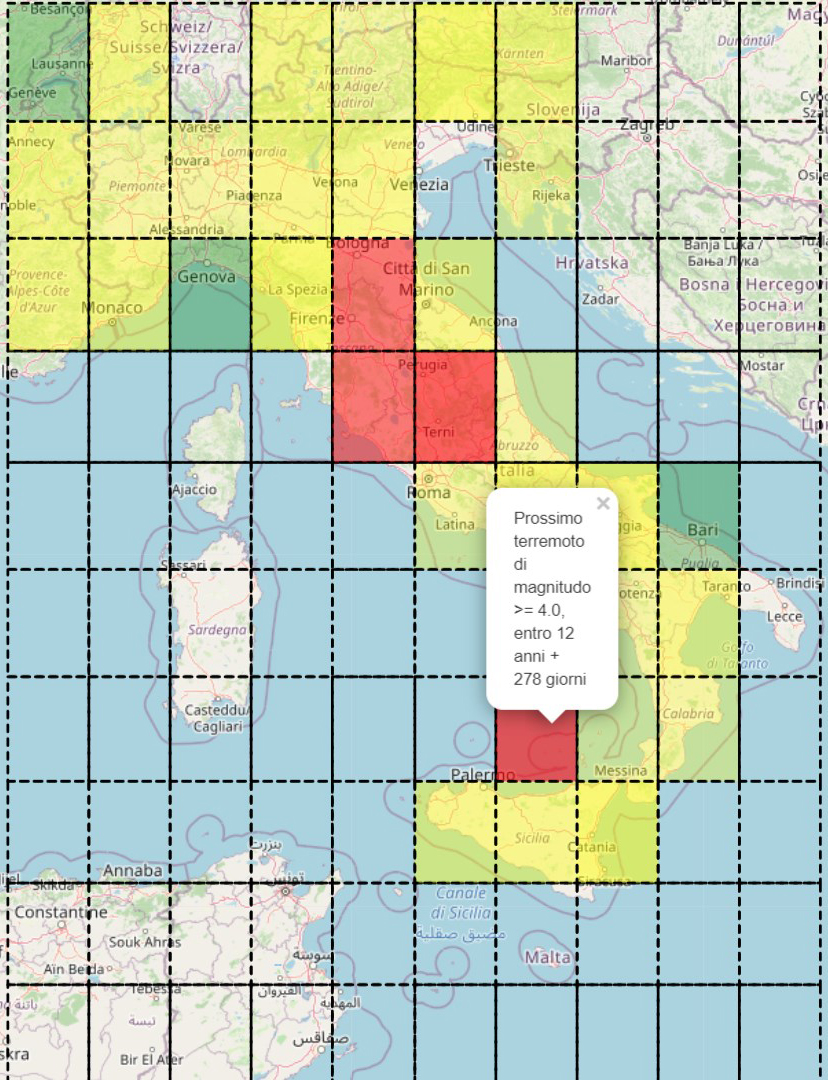
\includegraphics[width=0.600\textwidth]{images/10x10_mag4_12anniEvidenziato_CPTI15.jpg}
   \caption{Griglia 10x10 con DB CPTI15, magnitudo minima 4 evidenziata la cella con previsione pi\`u vicina}
   \label{fig:10x10_mag4_12anniEvidenziato}
\end{figure}

La prima che voglio analizzare \`e la Figura \ref{fig:10x10_mag4_12anniEvidenziato}. Questa \`e prodotta dall'input n = 10, x = 4 quindi avremo una griglia 10x10 che in base al criterio descritto sopra colora la mappa e ne rappresenta una stima in anni, che prevede con probabilit\`a del 75\% tra quanto avverr\`a il prossimo terremoto nella cella i-esima. In questo caso specifico prendiamo la cella colorata di rosso scuro, quella con numero minimo di giorni per i quali \`e previsto un terremoto con magnitudo $\ge$ 4, la cella in questione \`e la 7x7, vediamo come cliccandoci sopra si apre un popup che ci dice fra 12 anni + 278 giorni al massimo avverr\`a il prossimo terremoto con magnitudo $\ge$ 4, ora per verificare se la stima fatta dall'algoritmo ha dato esito positivo andiamo a utilizzare il programma descritto precedentemente che ci permette di verificarlo.

\begin{figure}[H]
   \centering
   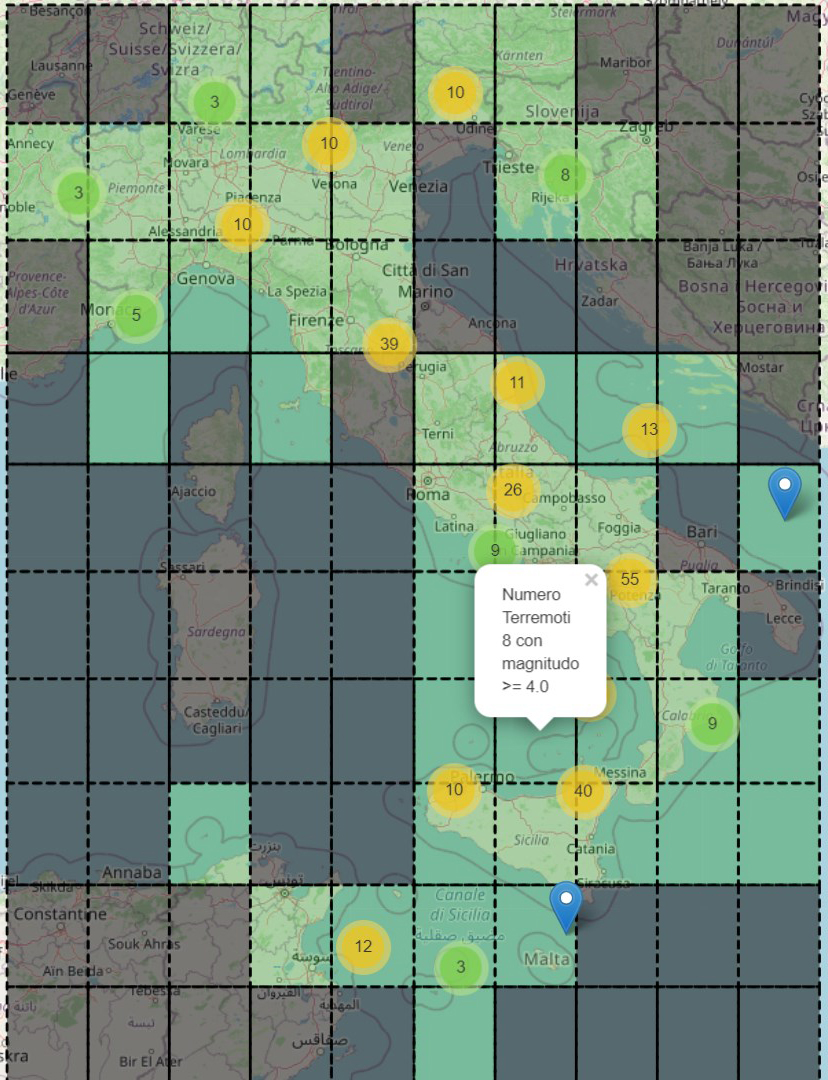
\includegraphics[width=0.600\textwidth]{images/10x10_mag4_12anniDopo_CPTI15.jpg}
   \caption{Griglia 10x10 con DB CPTI15, magnitudo minima 4 terremoti avvenuti dal 1981 al 1993}
   \label{fig:10x10_mag4_12anniDopo}
\end{figure}

Andando a cliccare sulla cella che abbiamo preso in considerazione, scopriamo che dal 1981 al 1993, ovvero nei 12 anni successivi ai dati che ho usato per stimare la previsione, ci sono stati 8 terremoti con magnitudo $\ge$ 4. Quindi l'esito dell'algoritmo \`e stato positivo. Ora voglio portare alla luce un fatto, sulle celle precedentemente colorate di rosso, gi\`a a 12 anni di distanza si sono registrati terremoti tranne che su una la 4x5. Vorrei prendere in analisi proprio questa, vedendo fra quanti anni l'algoritmo stima ci sar\`a il prossimo terremoto al massimo.

\begin{figure}[H]
   \centering
   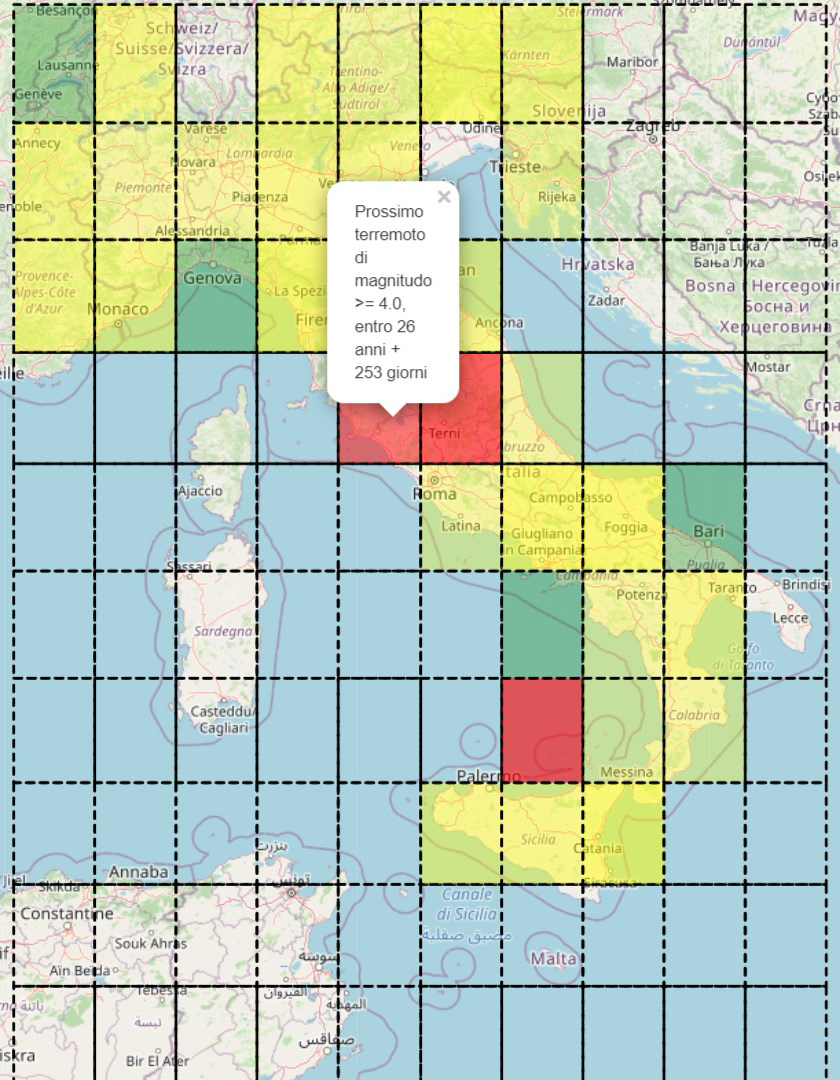
\includegraphics[width=0.600\textwidth]{images/10x10_mag4_26anniEvidenziato_CPTI15.jpg}
   \caption{Griglia 10x10 con DB CPTI15, magnitudo minima 4 evidenziata la cella con previsione subito successiva alla pi\`u vicina}
   \label{fig:10x10_mag4_26anniEvidenziato}
\end{figure}

Come si vede dalla Figura  \ref{fig:10x10_mag4_26anniEvidenziato} nella cella 4x5 la stima minima in anni \`e 26, quindi la griglia risultante del programma che verifica non pu\`o essere presa in considerazione, vado a generare una nuova griglia questa volta aumentando l'intervallo di anni da tenere in considerazione.

\begin{figure}[H]
   \centering
   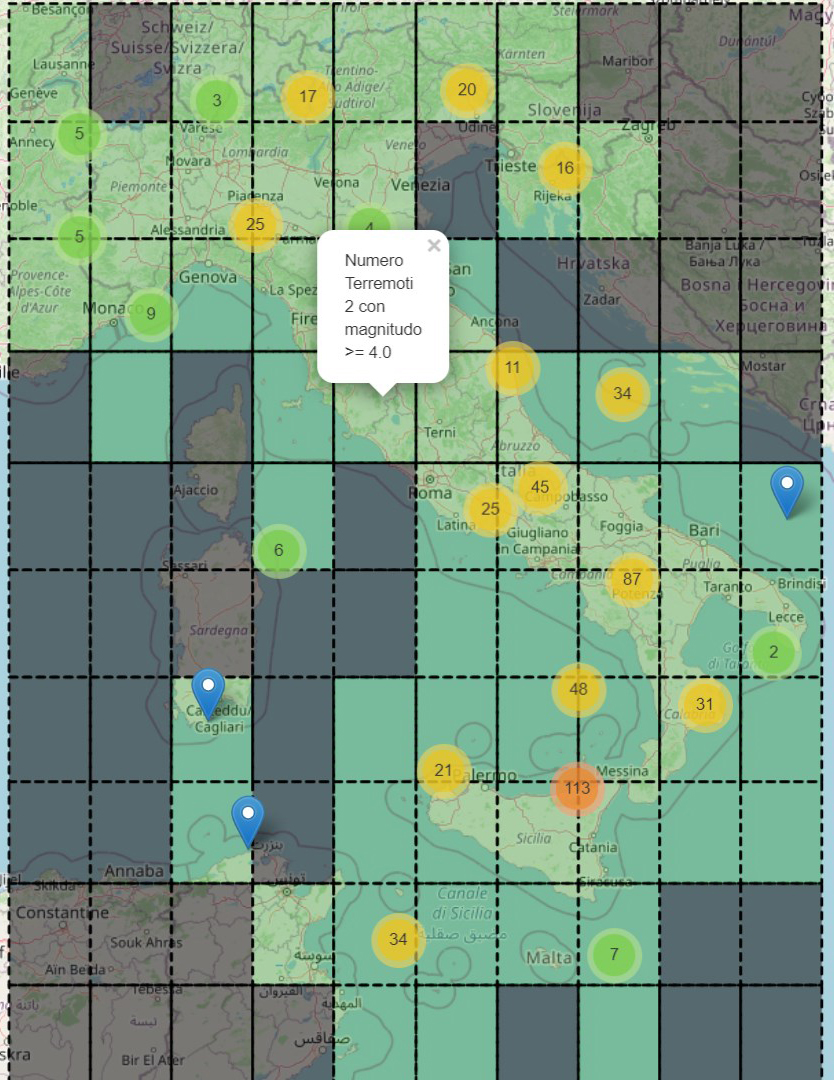
\includegraphics[width=0.600\textwidth]{images/10x10_mag4_26anniDopo_CPTI15.jpg}
   \caption{Griglia 10x10 con DB CPTI15, magnitudo minima 4 terremoti avvenuti dal 1981 al 2007}
   \label{fig:10x10_mag4_26anniDopo}
\end{figure}

La cella 4x5 risulta ora colorata di verde, infatti andando nel dettaglio riusciamo a vedere che dal 1981 al 2007 i terremoti avvenuti sono 2. Anche se il numero \`e piccolo anche questo risultato porta esito positivo dell'algoritmo. Come si vede dalle Figure \ref{fig:10x10_mag4_12anniDopo} e \ref{fig:10x10_mag4_26anniDopo} ci sono celle colorate in verde anche dove l'algoritmo non aveva calcolato una stima, questo avviene perch\'e in quelle celle non erano presenti dati storici o quelli presenti erano insufficienti, e quindi non hanno permesso la creazione della stima. Infatti quando le celle dell'output del programma basato sul secondo approccio sono trasparenti, significa che non ci sono stati pi\`u di 10 terremoti in quella cella superiori alla magnitudo x presa in considerazione, pertanto la stima non viene fatta. Questo evidenzia quanto sia importante avere a disposizione una grande mole di dati per far si che l'algoritmo porti risultati pi\`u precisi. Di seguito mostro graficamente altri esempi andando a prendere in considerazione una magnitudo pi\`u alta, quindi solitamente questo comporta un minor numero di dati storici a disposizione, in quanto terremoti con una magnitudo pi\`u alta avvengono pi\`u raramente (per nostra fortuna).

\begin{figure}[H]
   \centering
   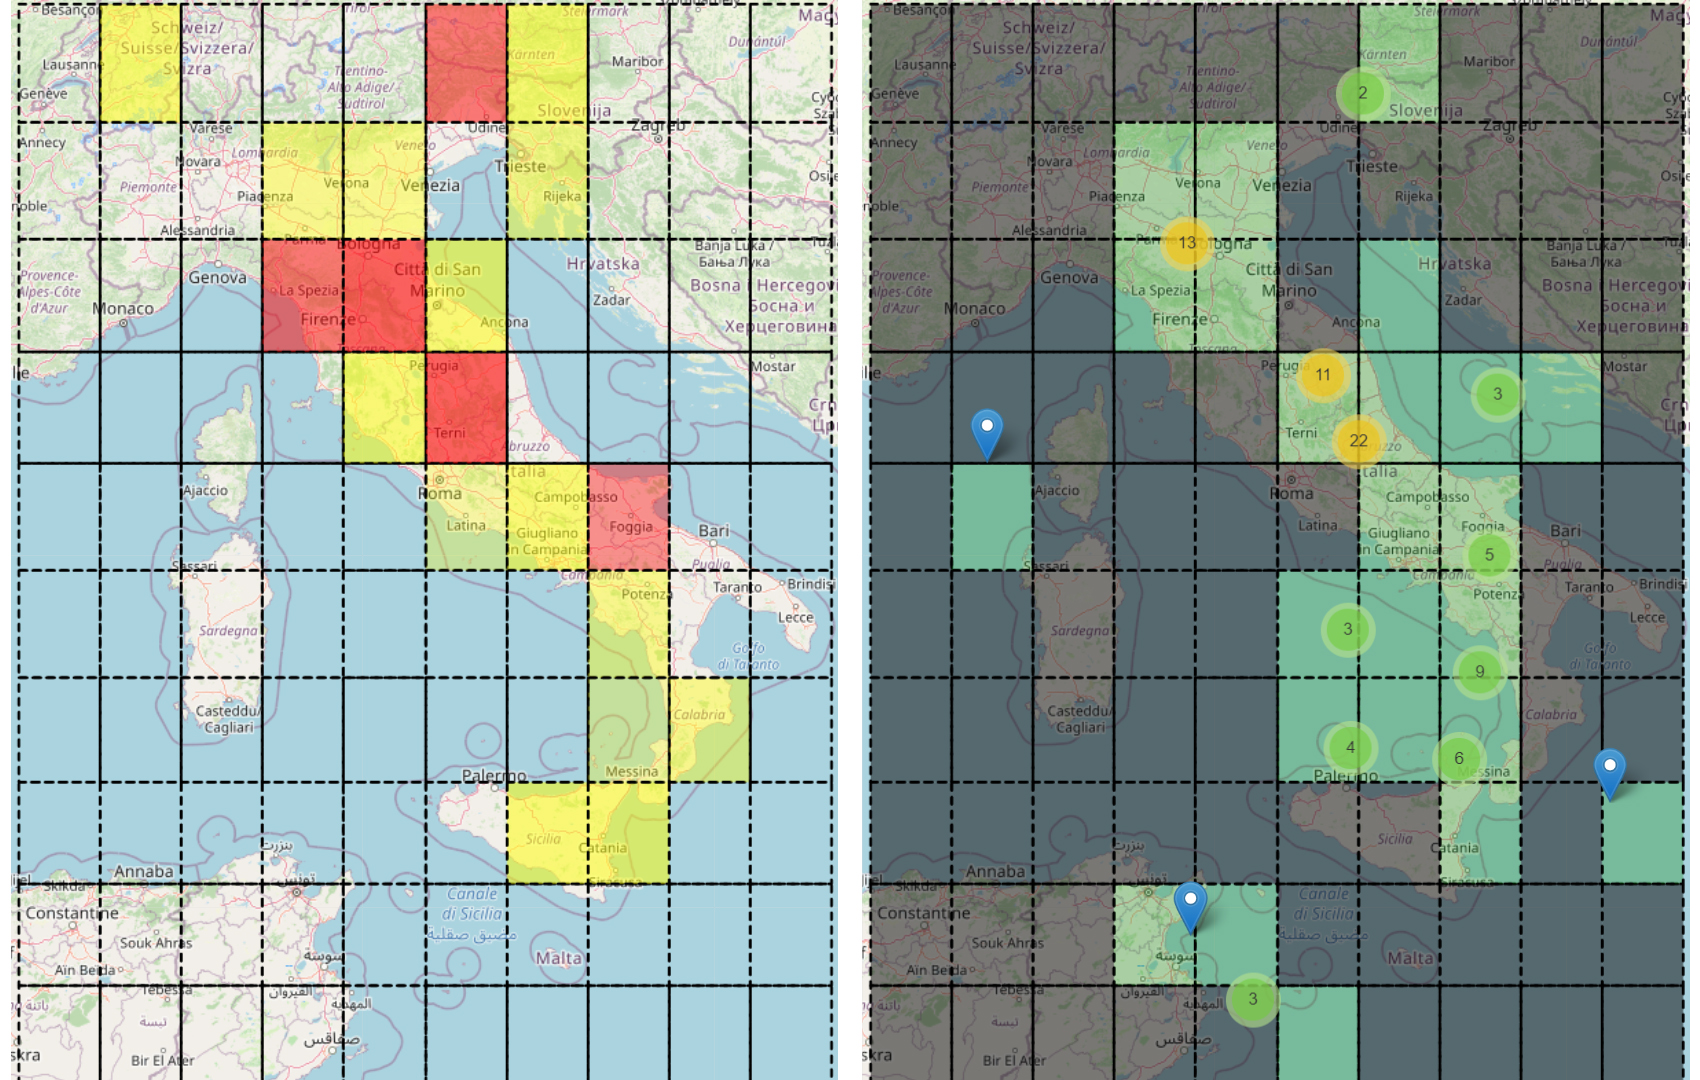
\includegraphics[width=0.835\textwidth]{images/10x10_mag5_confronto_36anniDopo_CPTI15.jpg}
   \caption{Griglia 10x10 con DB CPTI15, magnitudo minima 5, confrontato con terremoti avvenuti dal 1981 al 2017}
   \label{fig:10x10_mag5_36anniDopo}
\end{figure}

La cella con la previsione pi\`u vicina \`e la cella rossa nel centro Italia che riporta una previsione a 41 anni, mentre le celle gialle partono tutte da poco pi\`u di 100 anni, queste sono tutte previsioni a lungo termine, quindi non avendo a disposizione i dati oltre il 2017 posso confrontare la previsione soltanto con i terremoti avvenuti dal 1981 al 2017 che sono quindi i terremoti avvenuti fino a 36 anni dopo i dati utilizzati per la previsione. Come si vede dalla Figura \ref{fig:10x10_mag5_36anniDopo} nelle celle colorate di rosso dopo 36 anni sono gi\`a avvenuti dei terremoti, tranne che nella cella 1x6 dove la previsione mi dice 99 anni, quindi \`e una delle rosse pi\`u al limite, ovvero rientra quasi tra le celle gialle che partono da poco pi\`u di 100 anni.\\
Di seguito faccio ulteriori confronti con una griglia pi\`u dettagliata ovvero 15x15.

\begin{figure}[H]
   \centering
   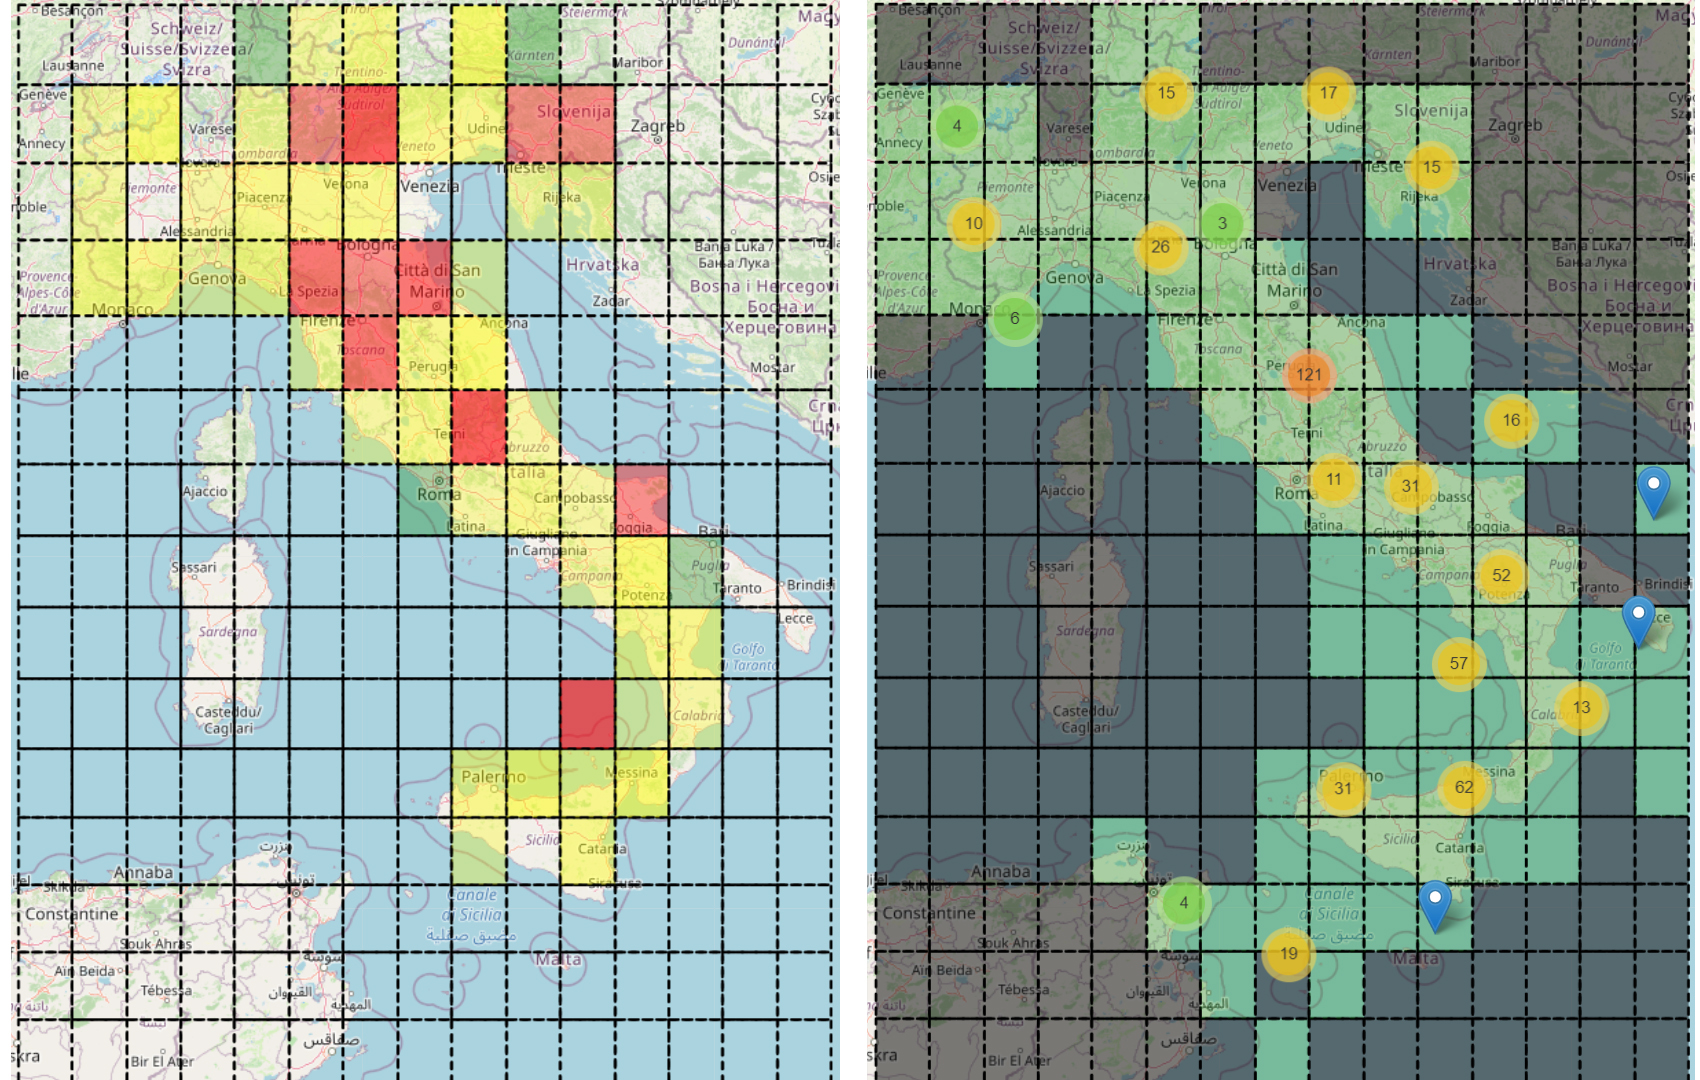
\includegraphics[width=0.835\textwidth]{images/15x15_mag4_confronto_18anniDopo_CPTI15.jpg}
   \caption{Griglia 15x15 con DB CPTI15, magnitudo minima 4, confrontato con terremoti avvenuti dal 1981 al 1999}
   \label{fig:15x15_mag4_18anniDopo}
\end{figure}

\begin{figure}[H]
   \centering
   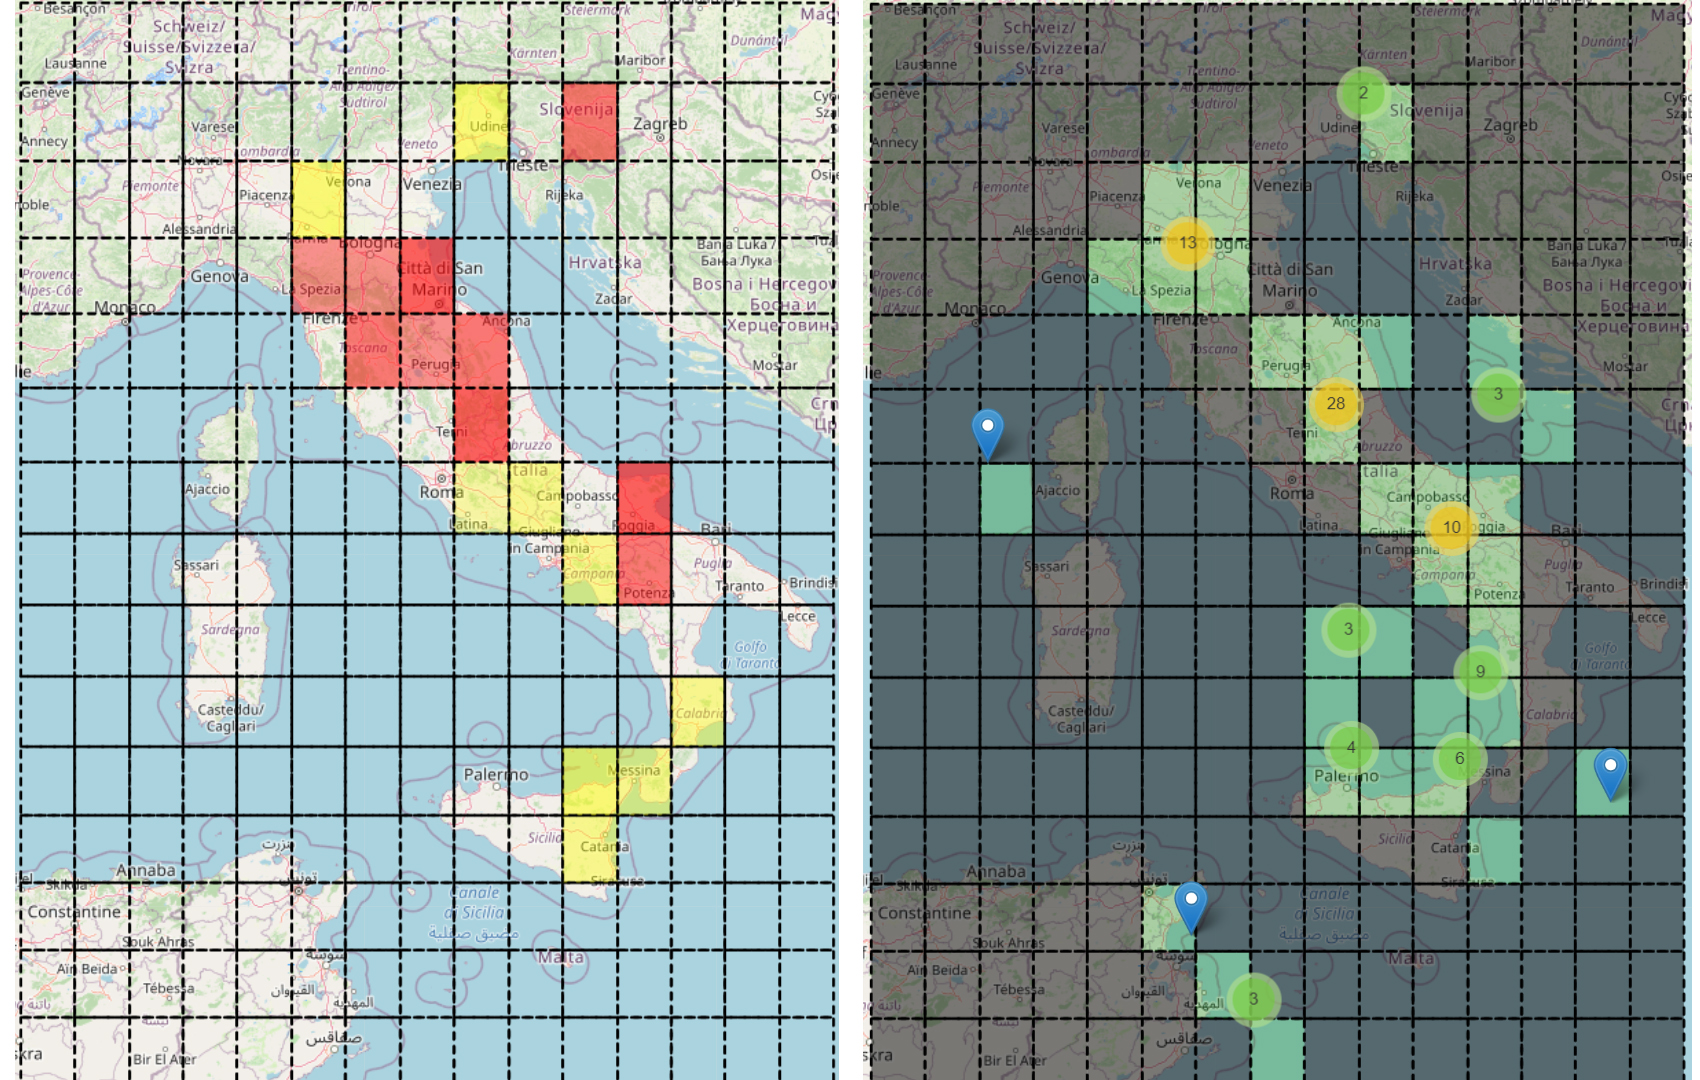
\includegraphics[width=0.835\textwidth]{images/15x15_mag5_confronto_36anniDopo_CPTI15.jpg}
   \caption{Griglia 15x15 con DB CPTI15, magnitudo minima 5, confrontato con terremoti avvenuti dal 1981 al 2017}
   \label{fig:15x15_mag5_36anniDopo}
\end{figure}

Anche in queste due ultime rappresentazioni grafiche dei risultati si vede come l'algoritmo funziona discretamente bene, prevedendo per la maggior parte delle celle i terremoti che avverranno entro una data limite. Nello specifico analizzando la Figura \ref{fig:15x15_mag4_18anniDopo} la cella rossa nel centro Italia \`e quella con la previsione pi\`u vicina, ovvero 18 anni a partire dal 1980, mentre le altre due subito successive, colorate di rosso scuro sono quelle nel nord e nel sud Italia, che rispettivamente hanno una previsione di 24 e 22 anni, in questo caso ho voluto confrontare con la mappa riportante i terremoti avvenuti dal 1981 al 1999 quindi prendendo come riferimento la cella nel centro Italia, e come si vede dalla foto l'esito per quella cella \`e stato positivo essendo avvenuti ben 44 terremoti di magnitudo $\ge$ 4. Anche per le altre due celle rosse gi\`a 18 anni dopo troviamo dei terremoti avvenuti in esse, e non solo, molte delle celle gialle sono state gi\`a colpite da terremoti con magnitudo $\ge$ 4 entro 18 anni. Per la Figura \ref{fig:15x15_mag5_36anniDopo} non entro nel dettaglio in quanto la previsione minima nella cella rosso scuro del centro Italia supera i 50 anni e la mappa di confronto come anche detto in precedenza non pu\`o superare i 36 anni, quindi lascio parlare la rappresentazione grafica.\\
Ometto l'analisi numerica dei risultati, in quanto risulterebbe scorretto affermare l'affidabilit\`a dell'algoritmo predittivo soltanto con i dati a disposizione, questo perch\'e la maggior parte delle celle nelle mappe in output dell'algoritmo, vanno fuori dal range nel quale \`e possibile fare verifiche con i dati a disposizione, quindi mi attengo al fatto di aver usato la formula derivante dalla disuguaglianza di Chebychev, pertanto a priori se come gi\`a detto, considero le rilevazioni empiriche sul passato assumendo che l'intervallo di tempo che intercorre fra due terremoti si comporti come una variabile aleatoria, posso affermare che il prossimo terremoto avverr\`a nella cella i-esima entro il numero di anni previsti dall'algoritmo con una probabilit\`a del 75\%.

\section{Strumenti utilizzati}\label{analisiDati}

Per analizzare i dati ho creato un programma scritto in linguaggio Python, linguaggio dinamico, semplice e flessibile che supporta la programmazione ad oggetti, strutturata e funzionale. Uno dei punti di forza di questo linguaggio \`e il poter importare una serie di librerie, ognuna delle quali pensata per uno specifico scopo di applicazione. Nel mio progetto saranno due le librerie che faranno da pilastri del programma:
\begin{itemize}
    \item \textit{Pandas} - La prima libreria essenziale ai fini del mio lavoro \`e un software scritto in linguaggio Python utilizzato per la manipolazione e l'analisi di grandi quantit\`a di dati, permette pertanto di leggere svariati formati con i quali solitamente si immagazzinano dati in formato digitale. I dati messi a disposizione dalla maggior parte degli enti, riguardanti i terremoti (e non), sono in formato .csv. Questo formato pu\`o essere immaginato (da noi persone) come una tabella, dove nella prima riga troviamo l'intestazione di ogni campo, per riconoscere i valori memorizzati nelle righe successive, ma per essere di facile comprensione per ogni programma i dati sono organizzati nella seguente maniera: suddivisi in righe, ogni riga utilizza una virgola come carattere di separazione tra un valore e il successivo e la prima riga contiene l'intestazione, ovvero il nome, dei valori rappresentati nelle righe successive;
    \item \textit{Folium} - I dati sarebbero inutili se non ci ponessimo l'obiettivo di rappresentarli e visualizzarli al meglio, per rispondere a ci\`o nasce questa libreria. Nel mio caso \`e stata utile per l'analisi visiva geospaziale dei dati, ovvero per la creazione di una mappa interattiva. Questo utilizzo \`e reso possibile grazie all'interazione tra \textit{Folium} e la famosa libreria \textit{Leaflet}\footnote{\`E la principale libreria JavaScript open source per mappe interattive ottimizzate per dispositivi mobili.}.
\end{itemize}
\chapter{Conclusioni}\label{conclusion}
In questo Capitolo vado a descrivere le conclusioni tratte dal mio lavoro ed a presentare possibili sviluppi futuri.\\
Quello che voglio evidenziare \`e quanto segue:\\
mi sono basato esclusivamente sui dati storici presenti nei cataloghi resi disponibili online. Ho ignorato gli aspetti tecnici, che possono essere i precursori di un terremoto, o anche le scosse di assestamento (che conseguono un forte terremoto) che per essere escluse hanno bisogno di funzioni matematiche, stabilite grazie all'aiuto di geologi, che conoscono il comportamento sismotettonico che avviene in una determinata area dopo un forte terremoto. Nonostrante ci\`o sono riuscito a ricavare una mappa, (vedi Figura \ref{fig:20x20vsWarningMap}) che rispecchia a grandi linee la mappa messa a disposizione dall'INGV. La differenza sostanziale sta nel fatto che per fare analisi di dati come ho fatto io, l'impiego di risorse economiche \`e inferiore a quello di altri tipi di ricerca, quindi apre molte possibilit\`a in quanto l'investimento non richiede una spesa esagerata. Quindi un aspetto molto importante che a volte viene lasciato da parte \`e la creazione di cataloghi concreti, contenenti molte informazioni sui dati storici e costantemente aggiornati. Quello che fa risaltare questa analisi \`e dare maggiore importanza ai cataloghi, ma soprattutto dare la possibilit\`a a chiunque di accedere ai dati attraverso delle queries di ricerca, limitando cos\`i direttamente la base dati che si andr\`a a scaricare.

\section{Sviluppi futuri}

I due programmi che ho sviluppato basati su due approcci differenti, utilizzano ognuno un criterio specifico da me scelto. Questo non preclude la possibilit\`a di andarli a migliorare, magari seguendo suggerimenti di persone qualificate nel campo della geofisica e vulcanologia. Questo per chiarire che soprattutto nel primo approccio mi baso su un criterio prettamente logico, per creare una stima di pericolosit\`a, ma con degli sviluppi successivi il programma potrebbe tirare fuori dei risultati pi\`u esaustivi, soprattutto basandosi su un appoccio pi\`u dettagliato.\\
Nel secondo approccio invece ho utilizzato il calcolo delle probabilit\`a tirando in gioco la formula risultante dalla disuguaglianza di Chebyshev, vedendo gli eventi passati come variabili aleatorie; anche in questo caso vedo delle possibili modifiche che tengono in considerazione metodi pi\`u precisi, magari gi\`a utilizzati in altri campi, che possono andare a modificare l'approccio.\\
Entrambi i programmi quindi sono dinamici in quanto \`e possibile, una volta definita la solida base che ho prontamente preparato, andare ad apportare delle modifiche agli algoritmi interni ai programmi, questo da ai due programmi una potenzialit\`a di crescita futura non indifferente.\\
Parlando invece dei cataloghi utilizzati e come gi\`a detto, se si rispettano le specifiche richieste dai programmi si potr\`a andare ad analizzare qualsiasi catalogo esportato nel giusto formato. Questo permette anche di creare una struttura che si mantiene aggiornata in automatico, ovvero che prenda dinamicamente i dati aggiornati in tempo reale e tracci delle stime sempre pi\`u accurate e aggiornate.\\
Un'altra possibilit\`a che deriva dalla presentazione fatta in precedenza dei programmi, \`e che il rettangolo definito in principio \`e anch'esso preso in input, quindi si potrebbe estendere l'analisi anche ad altre aree geografiche oltre l'Italia.\\
Come si evince gli sviluppi futuri sono molteplici, un altro degno di nota \`e la possibilit\`a di creazione di una interfaccia grafica, che eviti all'utente di interagire direttamente con il terminale passando gli argomenti in input a riga di comando, bens\`i di poter compilare un form, andando ad inserire li tutti gli input necessari per far girare il programma sulla propria richiesta. Naturalmente questa interfaccia pu\`o essere anche creata e messa a disposizione direttamente online, lasciando che i calcoli vengano fatti direttamente dal server WEB ospitante l'applicativo, che a quel punto sarebbe diventato un vero e proprio software pi\`u generale che permette la scelta dell'approccio o ancor di pi\`u ritorna i risultati di entrambi i programmi all'utente.
\chapter*{Ringraziamenti}
Voglio partire con il ringraziare il mio Relatore, il Prof. Francesco Pasquale, \`e stato sempre disponibile ogni qual volta avessi bisogno di un supporto tecnico o morale; anche in questo periodo di emergenza costretti a vederci soltanto via web (era una delle poche persone oltre la mia famiglia che vedevo). La sua cordialit\`a, precisione e competenza hanno fatto si che mi affidassi a lei per completare il mio percorso di studi nel migliore dei modi, la conferma ce l'ho avuta vedendo il lavoro di Tesi appagante che ne \`e venuto fuori (non che mi servisse una conferma).\\
Continuo con il ringraziare tutti i miei colleghi di corso che hanno condiviso con me questa splendida avventura, in particolar modo ne cito qualcuno:\\

\begin{itemize}
    \item Il brother, ho condiviso con te sin dal primo anno tutto, a partire dagli studi fino ad arrivare ai problemi della vita e i momenti di debolezza, ci siamo sempre fatti forza a vicenda ed \`e anche grazie al tuo supporto se ora sono arrivato fin qui, raggiungendo questo traguardo.
    \item Il gruppo JDMD, composto dal brother che ho citato sopra, da Ion e Lorenzo. Fantastici, mi avete accompagnato nell'esame di Ingegneria del Software, producendo un progetto bellissimo e degno di nota. Oltre a questo, ricordo con gioia i cappuccini e cornetti mangiati con te Ion prima di entrare a fare lezione di Algoritmi.
    \item Il gruppo di organizzatori dell'Hackathon 2019, un evento che mi ha portato gioia e gratificazione, Simone, Samir, Fede, Marcello e Manuel.
    \item Ringrazio poi Alessio, che se non fosse stato per te ero ancora fermo in uno degli scogli del mio corso di laurea, il tuo aiuto \`e stato essenziale, e ricorder\`o sempre la bella persona che sei.
    \item Tutto il Lab25A sempre presente per qualsiasi cosa, ragazzi fantastici che sono un punto di riferimento per il nostro corso di laurea in Informatica.
    \item Potrei mettere tra i miei colleghi universitari anche te, la mia splendida Donna che ho incontrato durante questo percorso, ma in quanto tale ti meriti uno spazio riservato $<$3, pertanto ti ringrazier\`o successivamente.
\end{itemize}

Voglio poi continuare con il ringraziare tutti i miei amici, che mi hanno incoraggiato sin dall'inizio per portare a termine questo percorso intrapreso, anche in questo caso ne cito qualcuno:

\begin{itemize}
    \item Raffo, quel giorno, in quel parcheggio.. incontrare un amico di vecchia data e scoprire che anche tu come me avevi deciso, un po' in ritardo di intraprendere questo percorso formativo offerto dall'Universit\`a \`e stata una gioia. Abbiamo condiviso molti momenti insieme e te ne sono grato, perch\'e ogni momento \`e stato tempo ben speso.
    \item Davidello, una delle persone con cui ho condiviso moltissimo tempo soprattutto durante il periodo che precedeva la sessione, quando le lezioni erano terminate e si doveva ripassare, tu sei stato sempre presente mi hai fatto compagnia nello studio. Ma oltre l'Universit\`a ti ringrazio di essermi sempre vicino anche nella vita.
    \item Come dimenticare Ganega, \`e soltanto grazie a te che ingranai la marcia giusta, tu mi diedi l'aiuto necessario per superare l'esame di Analisi Matematica, primo grande scoglio. \`E stato un piacere farmi spiegare le cose da te, una persona preparata e competente che mi ha avvantaggiato molto. Dopo aver visto gli immediati risultati positivi gi\`a al primo Appello, ebbi conferma di quanto fu utile il tuo aiuto. Anche con te i ringraziamenti non si limitano a questo ma ti ringrazio per i bei momenti passati insieme, soprattutto le giornate al poligono per scaricare la tensione esplodendo un po' di colpi.
    \item Tutto il gruppo di amici splendidi che ho sin da quando sono piccolo, non potrei chiedere di meglio, siete la fortuna pi\`u grande che questa vita mi ha regalato. Parlo di Lele, Daniele, Riccardo, Andrea, Marcello e Sergio.
    \item Ringrazio la mia sorella non di sangue, Simona, che anche se durante il mio percorso era gi\`a alla conclusione del suo (bell'amica, mica mi aspetta..) ha saputo sostenermi e consigliarmi, ma anche farmi passare belle giornate spensierate (ad esempio sulla neve.. forse li il belle vale solo per me) che sono sempre utili per staccare dallo studio.
    \item Ringrazio i miei amici Fabio, Alessandro e Chiara, che con la vostra presenza avete sempre migliorato le mie giornate!
    \item Martina, Luca, Emanuele, Danilo, ecc. i miei amici abruzzesi, avete accompagnato da sempre le mie estati in quel fantastico posto, del quale ringrazio tutti gli abitanti parenti e non.
    \item Massimo, non mi ero dimenticato di te non iniziare ad agitarti, anche a te vanno i miei ringraziamenti, mi ricordo le spiegazioni essenziali per superare l'esame di Probabilit\`a. Ma soprattutto ricordo i tantissimo momenti fuori dalla vita universitaria, hai sempre saputo farmi svagare al meglio! Approfitto per ringraziare quel tuo coinquilino pazzo che mi \`e stato simpatico sin da subito, Fede.
\end{itemize}
\`E ora arrivato il momento di ringraziare te amore mio! La mia Fatima. Quando ho cominciato l'Universit\`a non ho pensato alla possibilit\`a di trovare l'amore, anche perch\'e ho deciso di studiare Informatica, ed \`e risaputo che ad Informatica le Donne sono assai rare. Invece ho incontrato te, la donna che ha reso questo ultimo anno della mia vita fantastico, spero di avere un bel futuro e spero di averlo insieme a te. Ti voglio ringraziare per essermi stata sempre vicina, per avermi sempre supportato e sopportato, per avermi dato coraggio nei momenti bui e forza quando ne avevo bisogno.\\
Infine voglio ringraziare voi, la mia splendida famiglia, che mi ha appoggiato quando ho deciso di intraprendere questo percorso, anche se questo comportava il lasciare il lavoro per dedicarmi a tempo pieno nello studio, siete stati subito d'accordo della mia scelta, supportandomi economicamente e dandomi la possibilit\`a di formarmi e di arrivare dove sono ora. Siete la famiglia migliore che si possa desiderare, sempre disposti ad aiutare senza chiedere mai nulla in cambio, mi avete dato sempre amore e spero di ripagarvi per tutta la vita con il doppio se non il triplo dell'amore ricevuto. Voglio includere nella mia famiglia anche voi, la mia famiglia adottiva, Sonia Claudio, Luca e Simona. Grazie per esserci sempre stati.\\
Non \`e vero non ho concluso, c'\`e una persona che ho deciso di ringraziare per ultima, non voglio fare preferenze, anche perch\'e gi\`a ti ho ringraziato nella famiglia, ma volevo dedicare a te questa Laurea Padre. \`E soltanto grazie alla tua fiducia che mi hai sempre dato che sono qui ora, ho creduto in me stesso, tornando indietro ti dico che probabilmente non mi ci sarei mai visto a possedere una Laurea, e invece eccomi qui. Probabilmente la fiducia che mi hai dato e che mi dai tutt'ora \`e pi\`u della fiducia che mi do io stesso. Quindi ti ringrazio per essere come sei, non potrei pretendere un padre migliore di te. Dedico quindi a te questo traguardo e ti ringrazio per avermi sempre sostenuto, ti voglio bene.
\listoffigures
\addcontentsline{toc}{chapter}{Elenco delle figure}
\bibliographystyle{plain}
\bibliography{bibliografia}

\end{document}
